\documentclass[10pt,a4paper]{article}
\usepackage[utf8]{inputenc}
\usepackage[T1]{fontenc}
\usepackage{amsmath}
\usepackage{amsfonts}
\usepackage{amssymb}
\usepackage{graphicx}
\usepackage{listings}
\usepackage{float}
\usepackage{subcaption}
\usepackage[labelformat=parens,labelsep=quad,skip=3pt]{caption}


\begin{document}
	\title{Homework 2 - Using Interrupts}
	\makeatletter
	
	\author{Zackary McClamma\thanks{University of Dayton}
		\thanks{Dept. of Electrical and Computer
			Engineering, University of Dayton, 300 College Park, Dayton, OH
			45469-0226, U.S.A. E-mail:
			mcclammaz1@udayton.edu}}
	
	\makeatother
	
	\date{\today}
	
	\maketitle
	\section{Introduction}
	In assignment consisted of configuring the NIOS II Processor in QuartusPrime and adding the 2 of the 7-segment displays and a button as peripherals. It also included creating software that would display the values 01-12 on the two 7-segment displays Figure \ref{fig:disp} by using an interrupt to iterate the value on the display whenever the button is pressed. This assignment also requiered the use of SignalTap to measure the latency of the interrupt which the  results of can be seen in Figure \ref{la10c}.
	
	\section{System Design}
	This system is very similar to the system designed in the first homework assignment, with two major differences. First in this assignemnt a second 7-Segment display was added, and second but most importantly, the button in this assignment uses an interrupt as opposed to polling in the previous assignment. The process is defined in \ref{block} below. In the figure the blue arrows indicate VHDL code, the red arrows indicate C code, and the green arrows indicate that both VHDL and C are being transmitted.  
	\begin{figure}
		\centering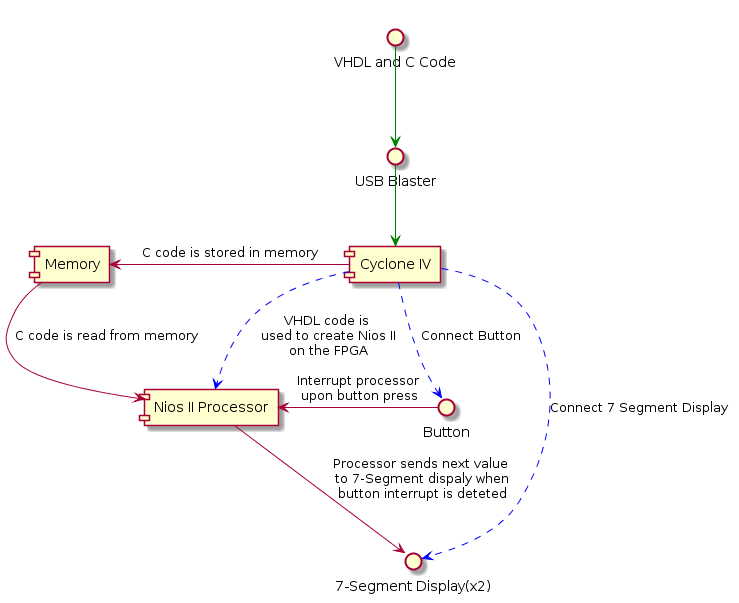
\includegraphics[width=15cm]{HW2_Block.png}
		\caption{Embedded System Block Diagram}
		\label{block}
	\end{figure}
	
	\section{Theory of Operation}
	The basic idea of this system is that the 7-segment display iterates through the values (01-12), with the value being incremented every time the button (KEY3) is pressed. When the button is pressed it sends an interrupt signal to the processor. The processor then saves its current state and immediately loads the interrupt service routine. The count value is then incremented and the button is reset back to its default state and the processor then reloads its state from before the interrupt signal was received.
	
	\section{Results}
		\subsection{Photos of Working System}
		\begin{figure}[H]

			\begin{subfigure}{3cm}
				\centering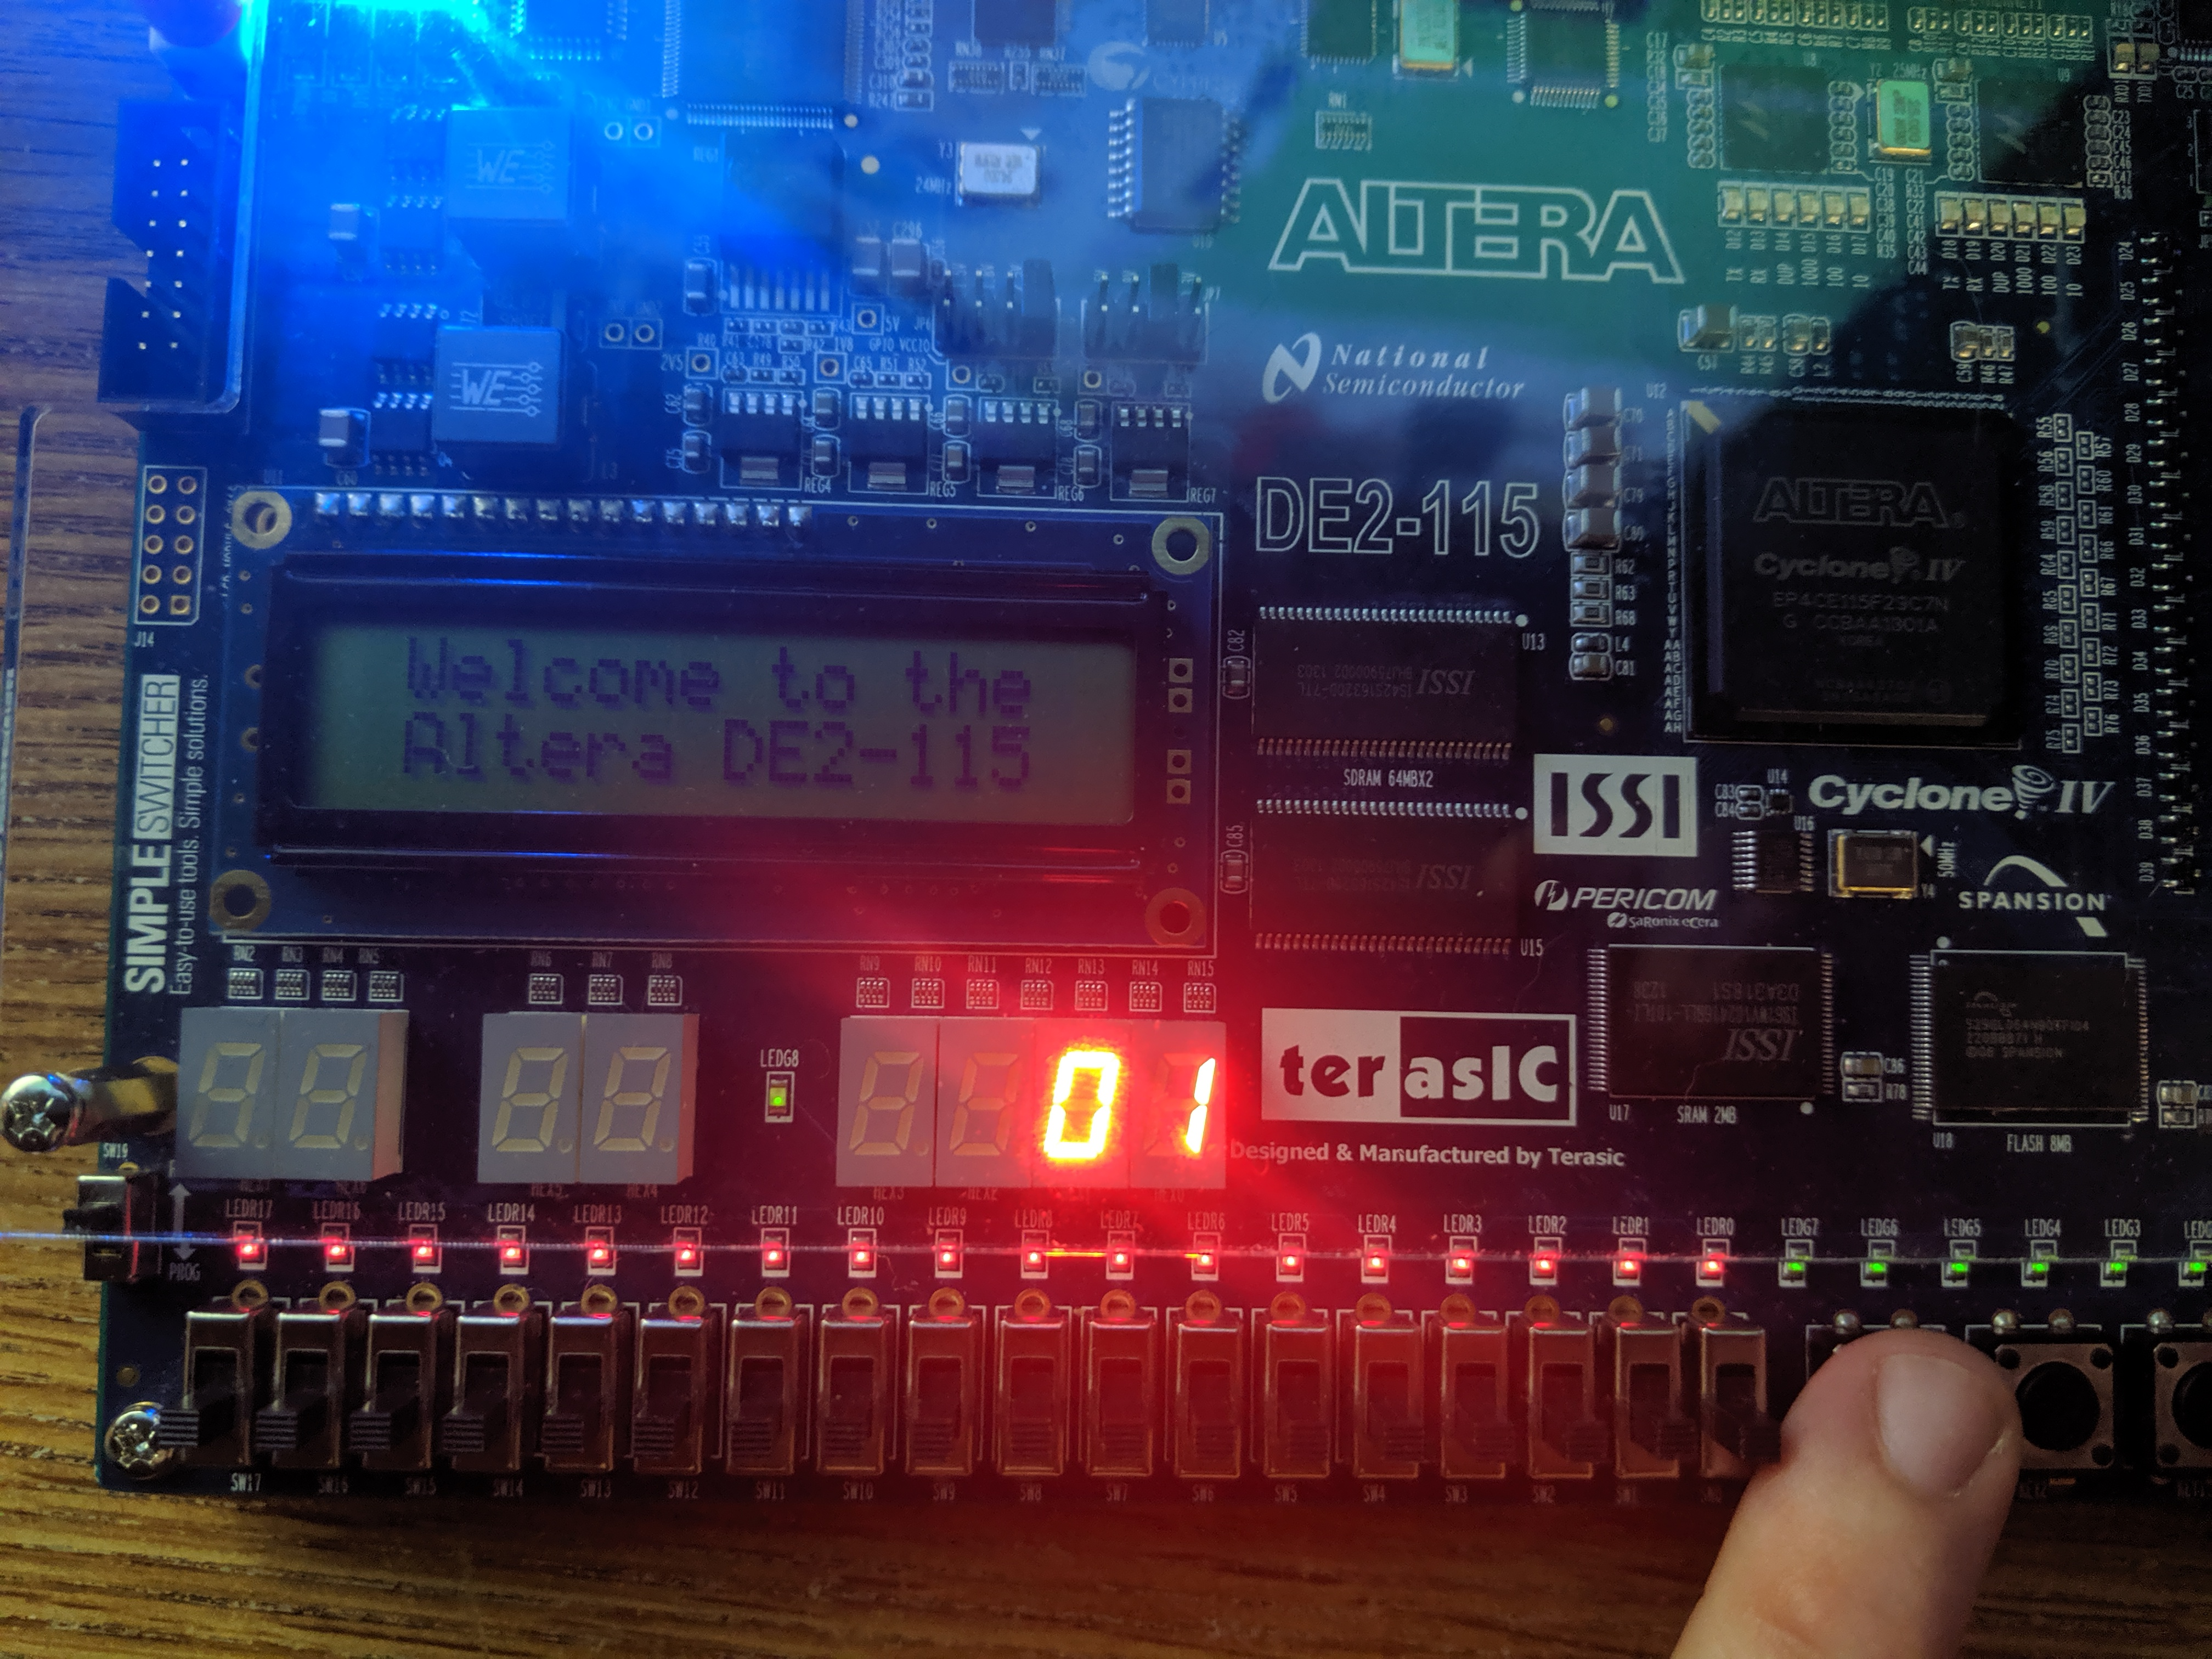
\includegraphics[width=3cm]{Display1.jpg}
				\caption{Display 1}
			\end{subfigure}
			\begin{subfigure}{3cm}
				\centering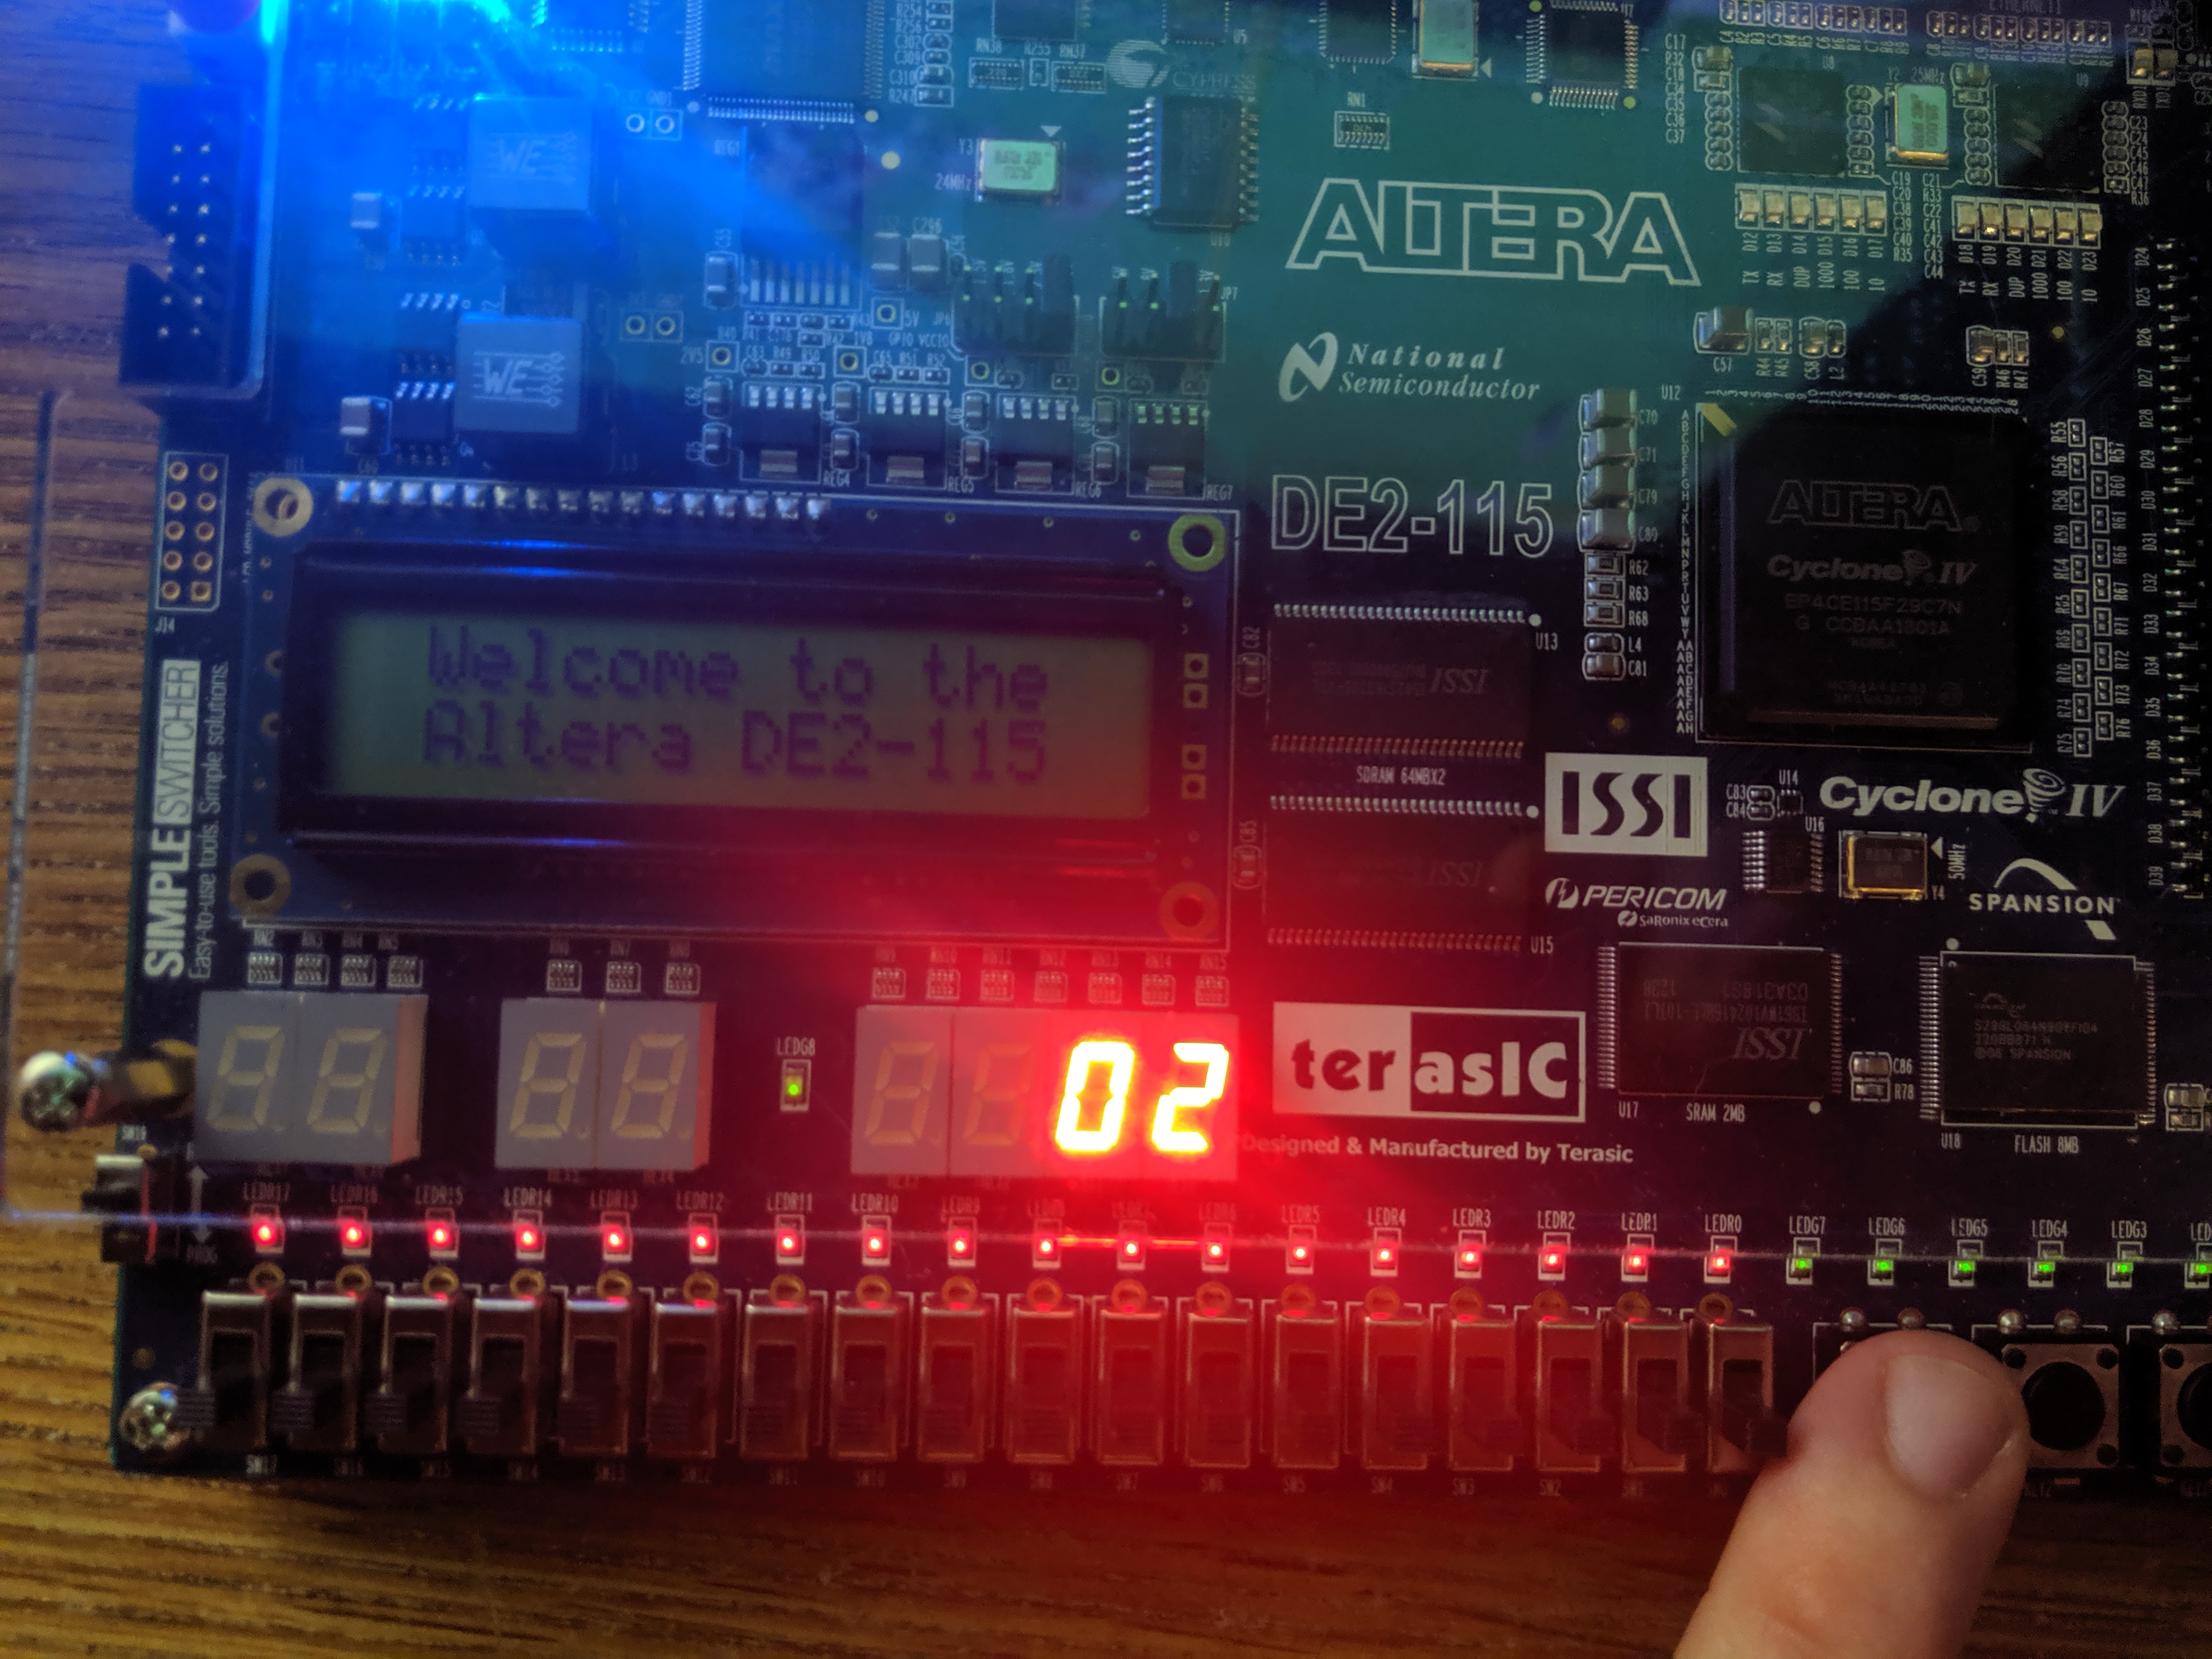
\includegraphics[width=3cm]{Display2.jpg}
				\caption{Display 2}
			\end{subfigure}
			\begin{subfigure}{3cm}
				\centering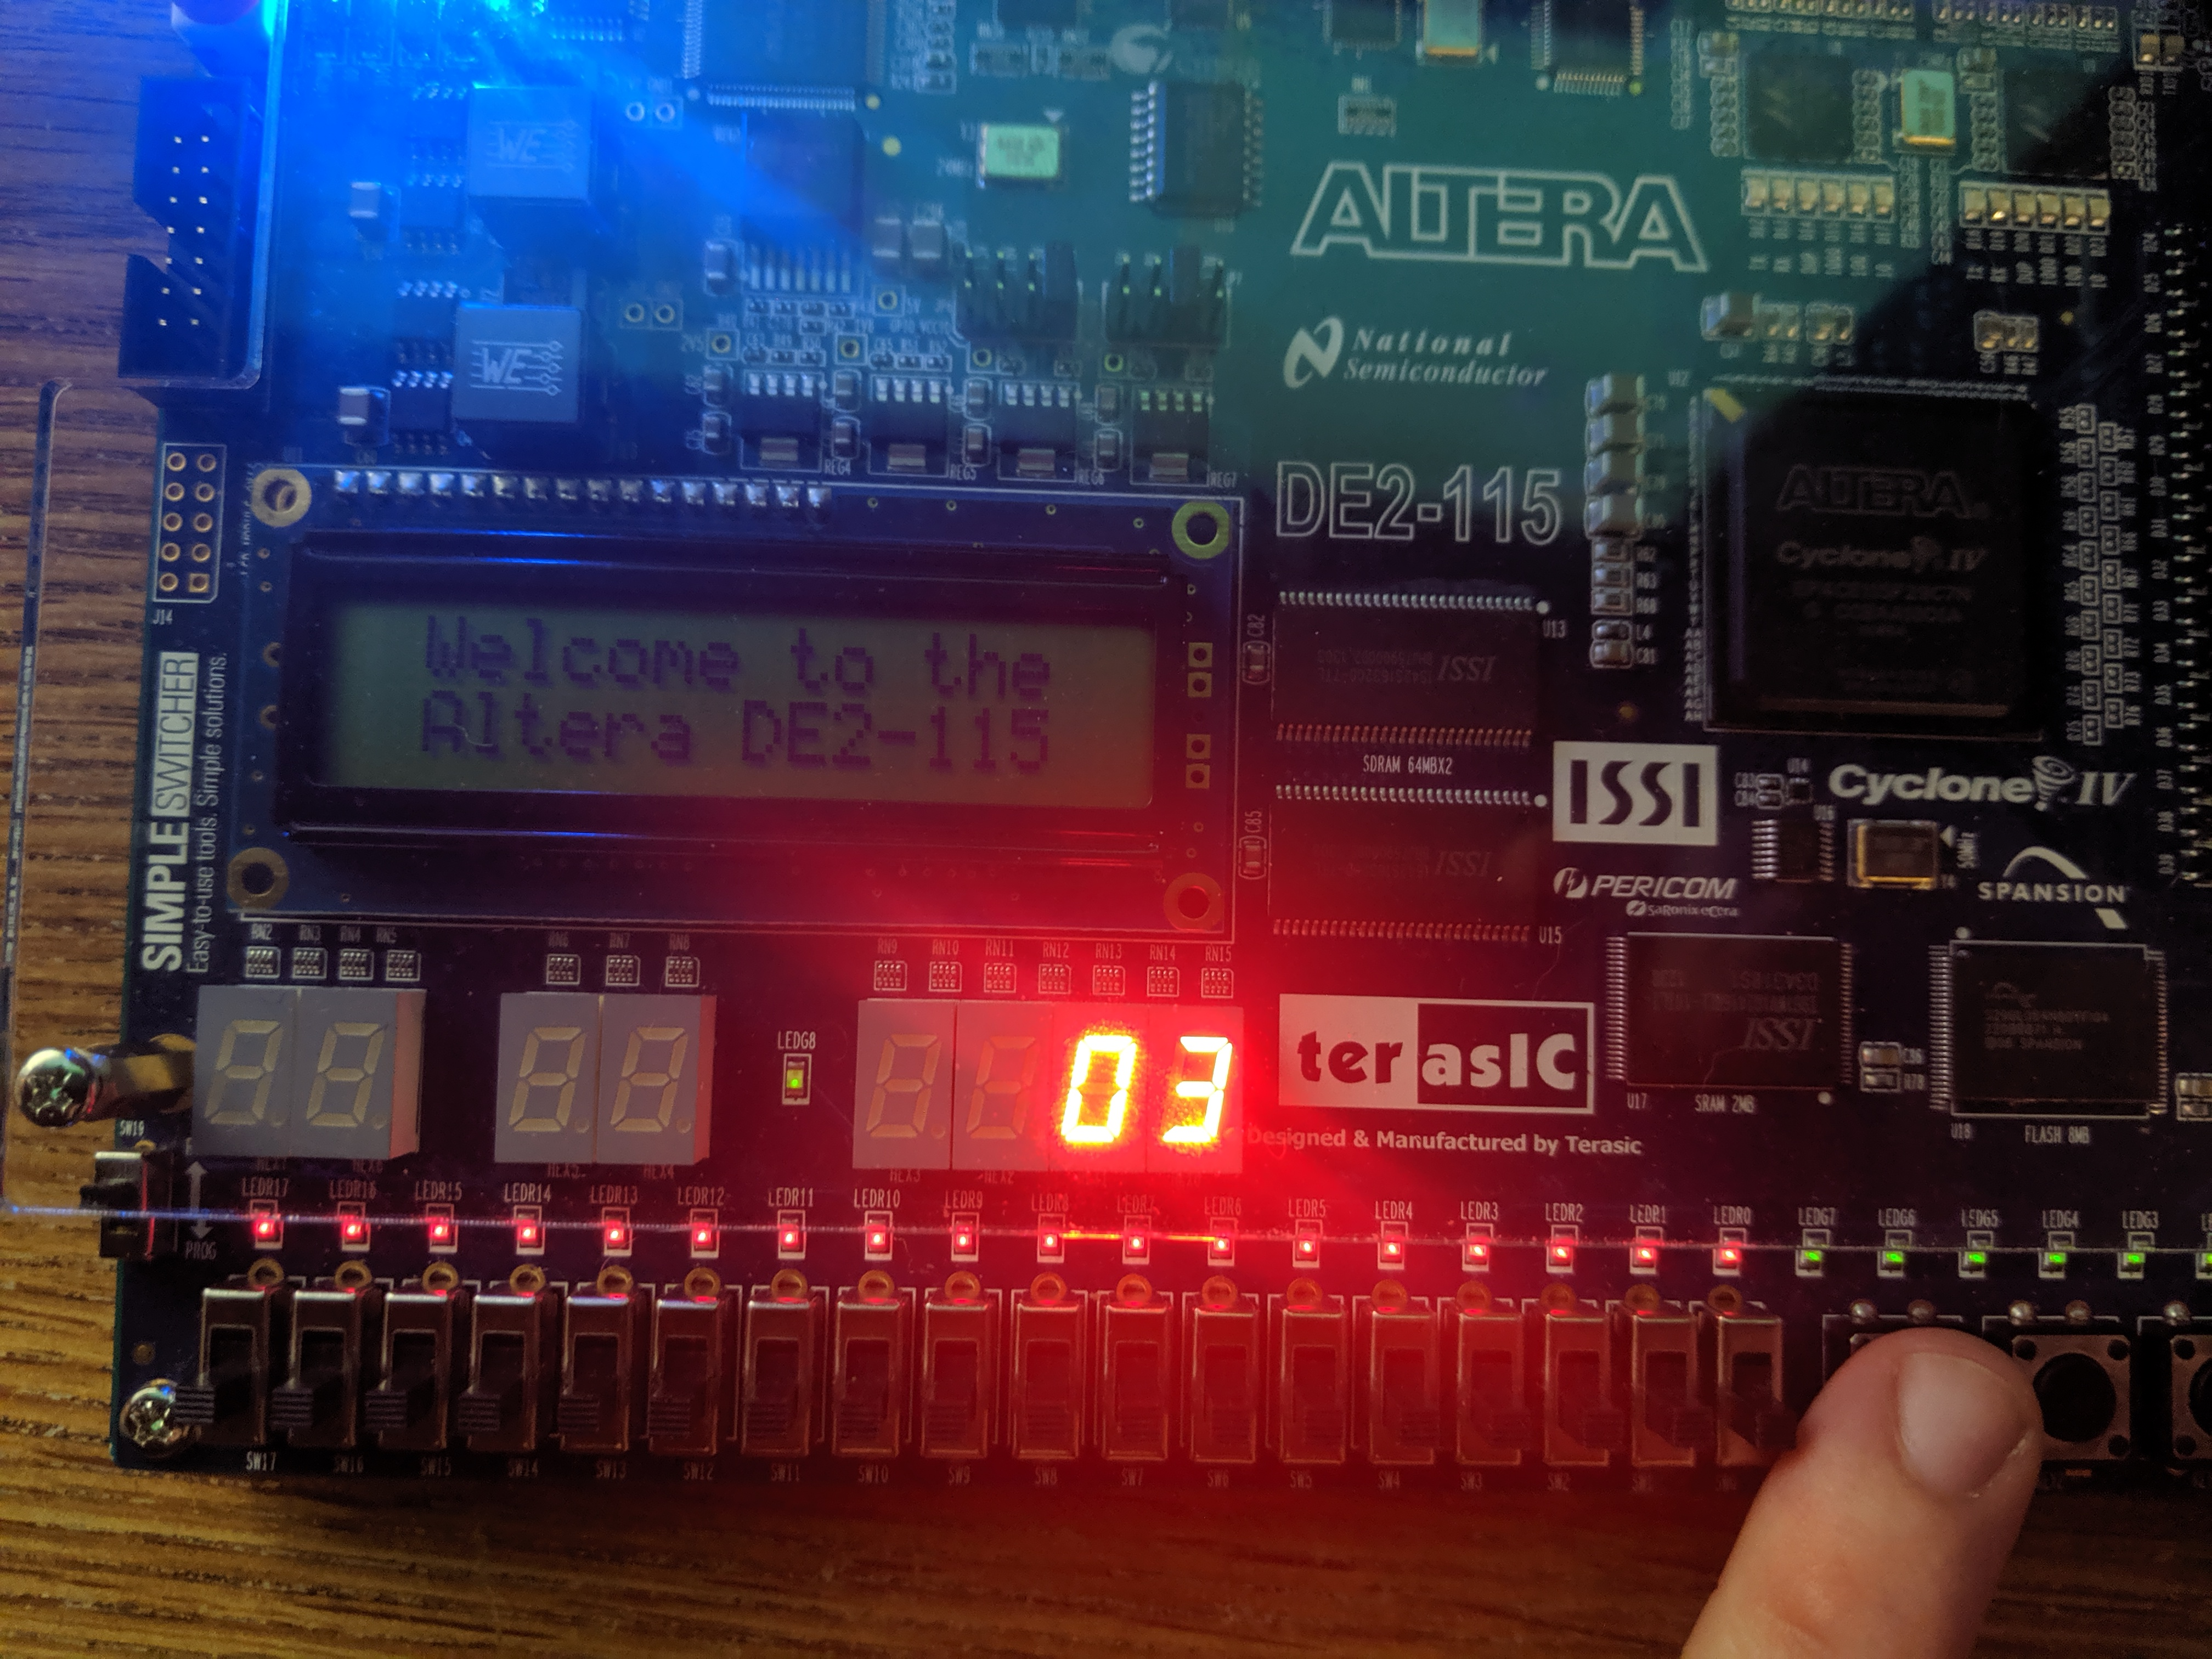
\includegraphics[width=3cm]{Display3.jpg}
				\caption{Display 3}
			\end{subfigure}
		
			\begin{subfigure}{3cm}
				\centering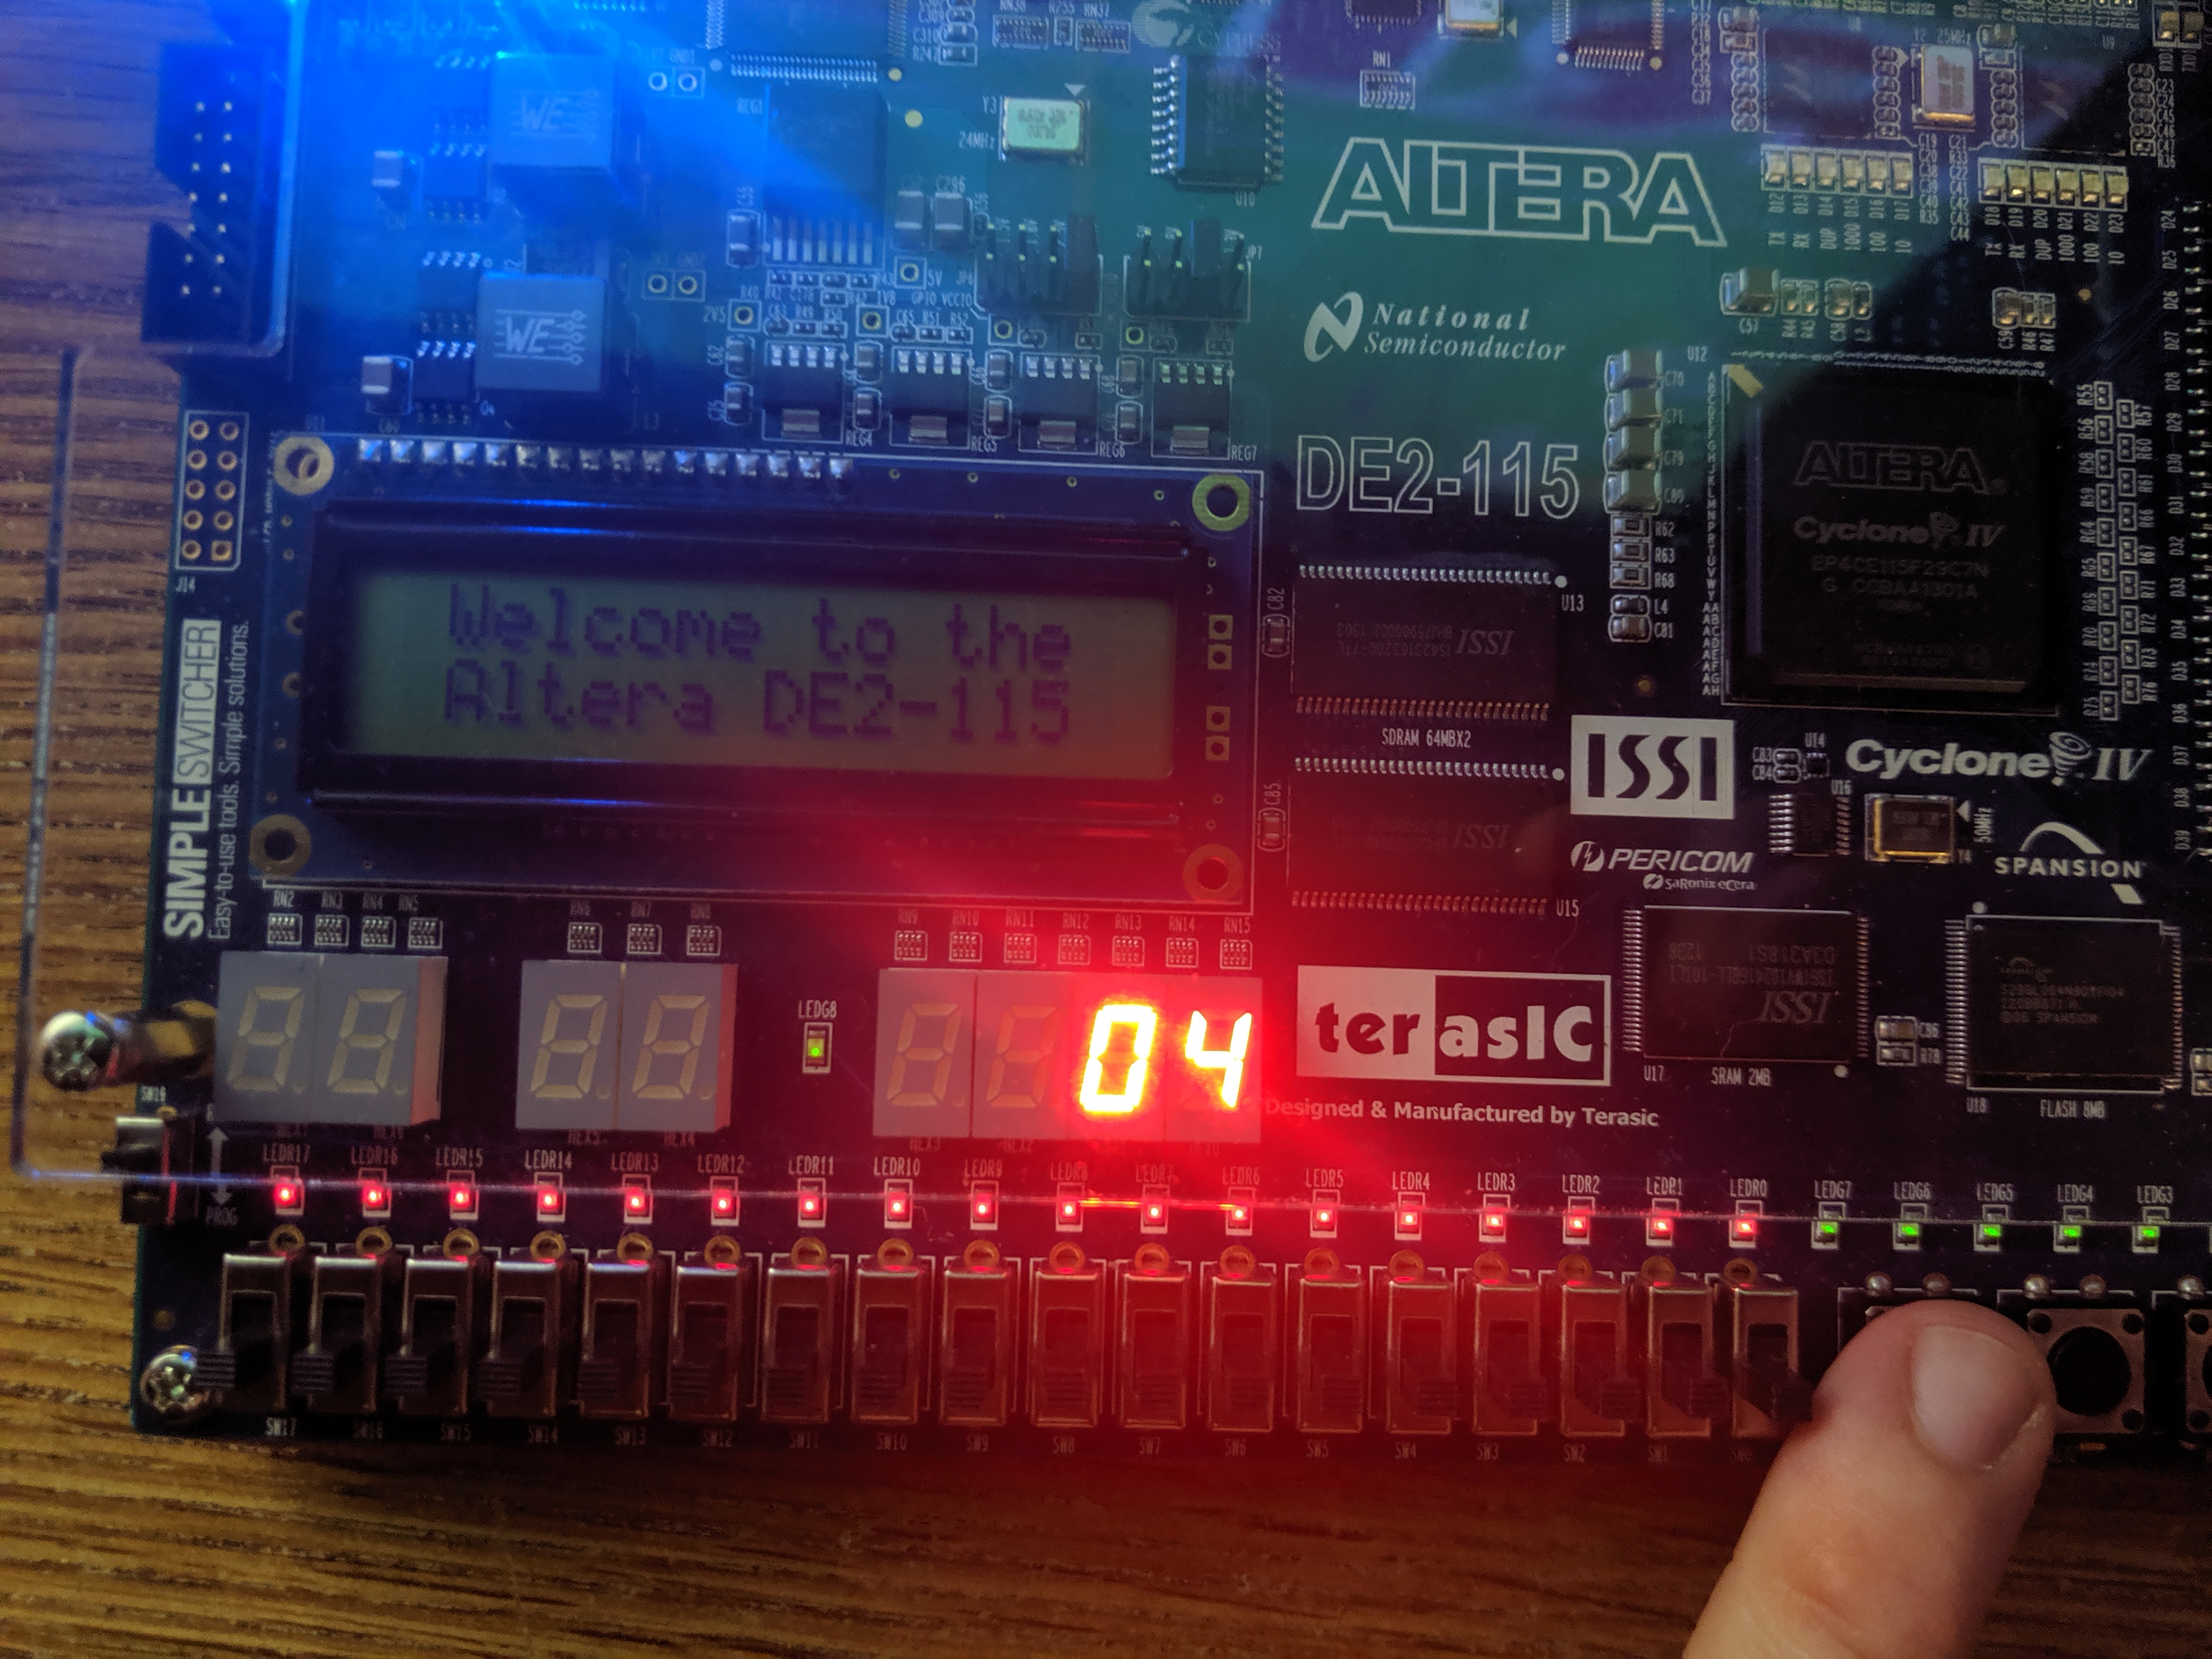
\includegraphics[width=3cm]{Display4.jpg}
				\caption{Display 4}
			\end{subfigure}	
			\begin{subfigure}{3cm}
				\centering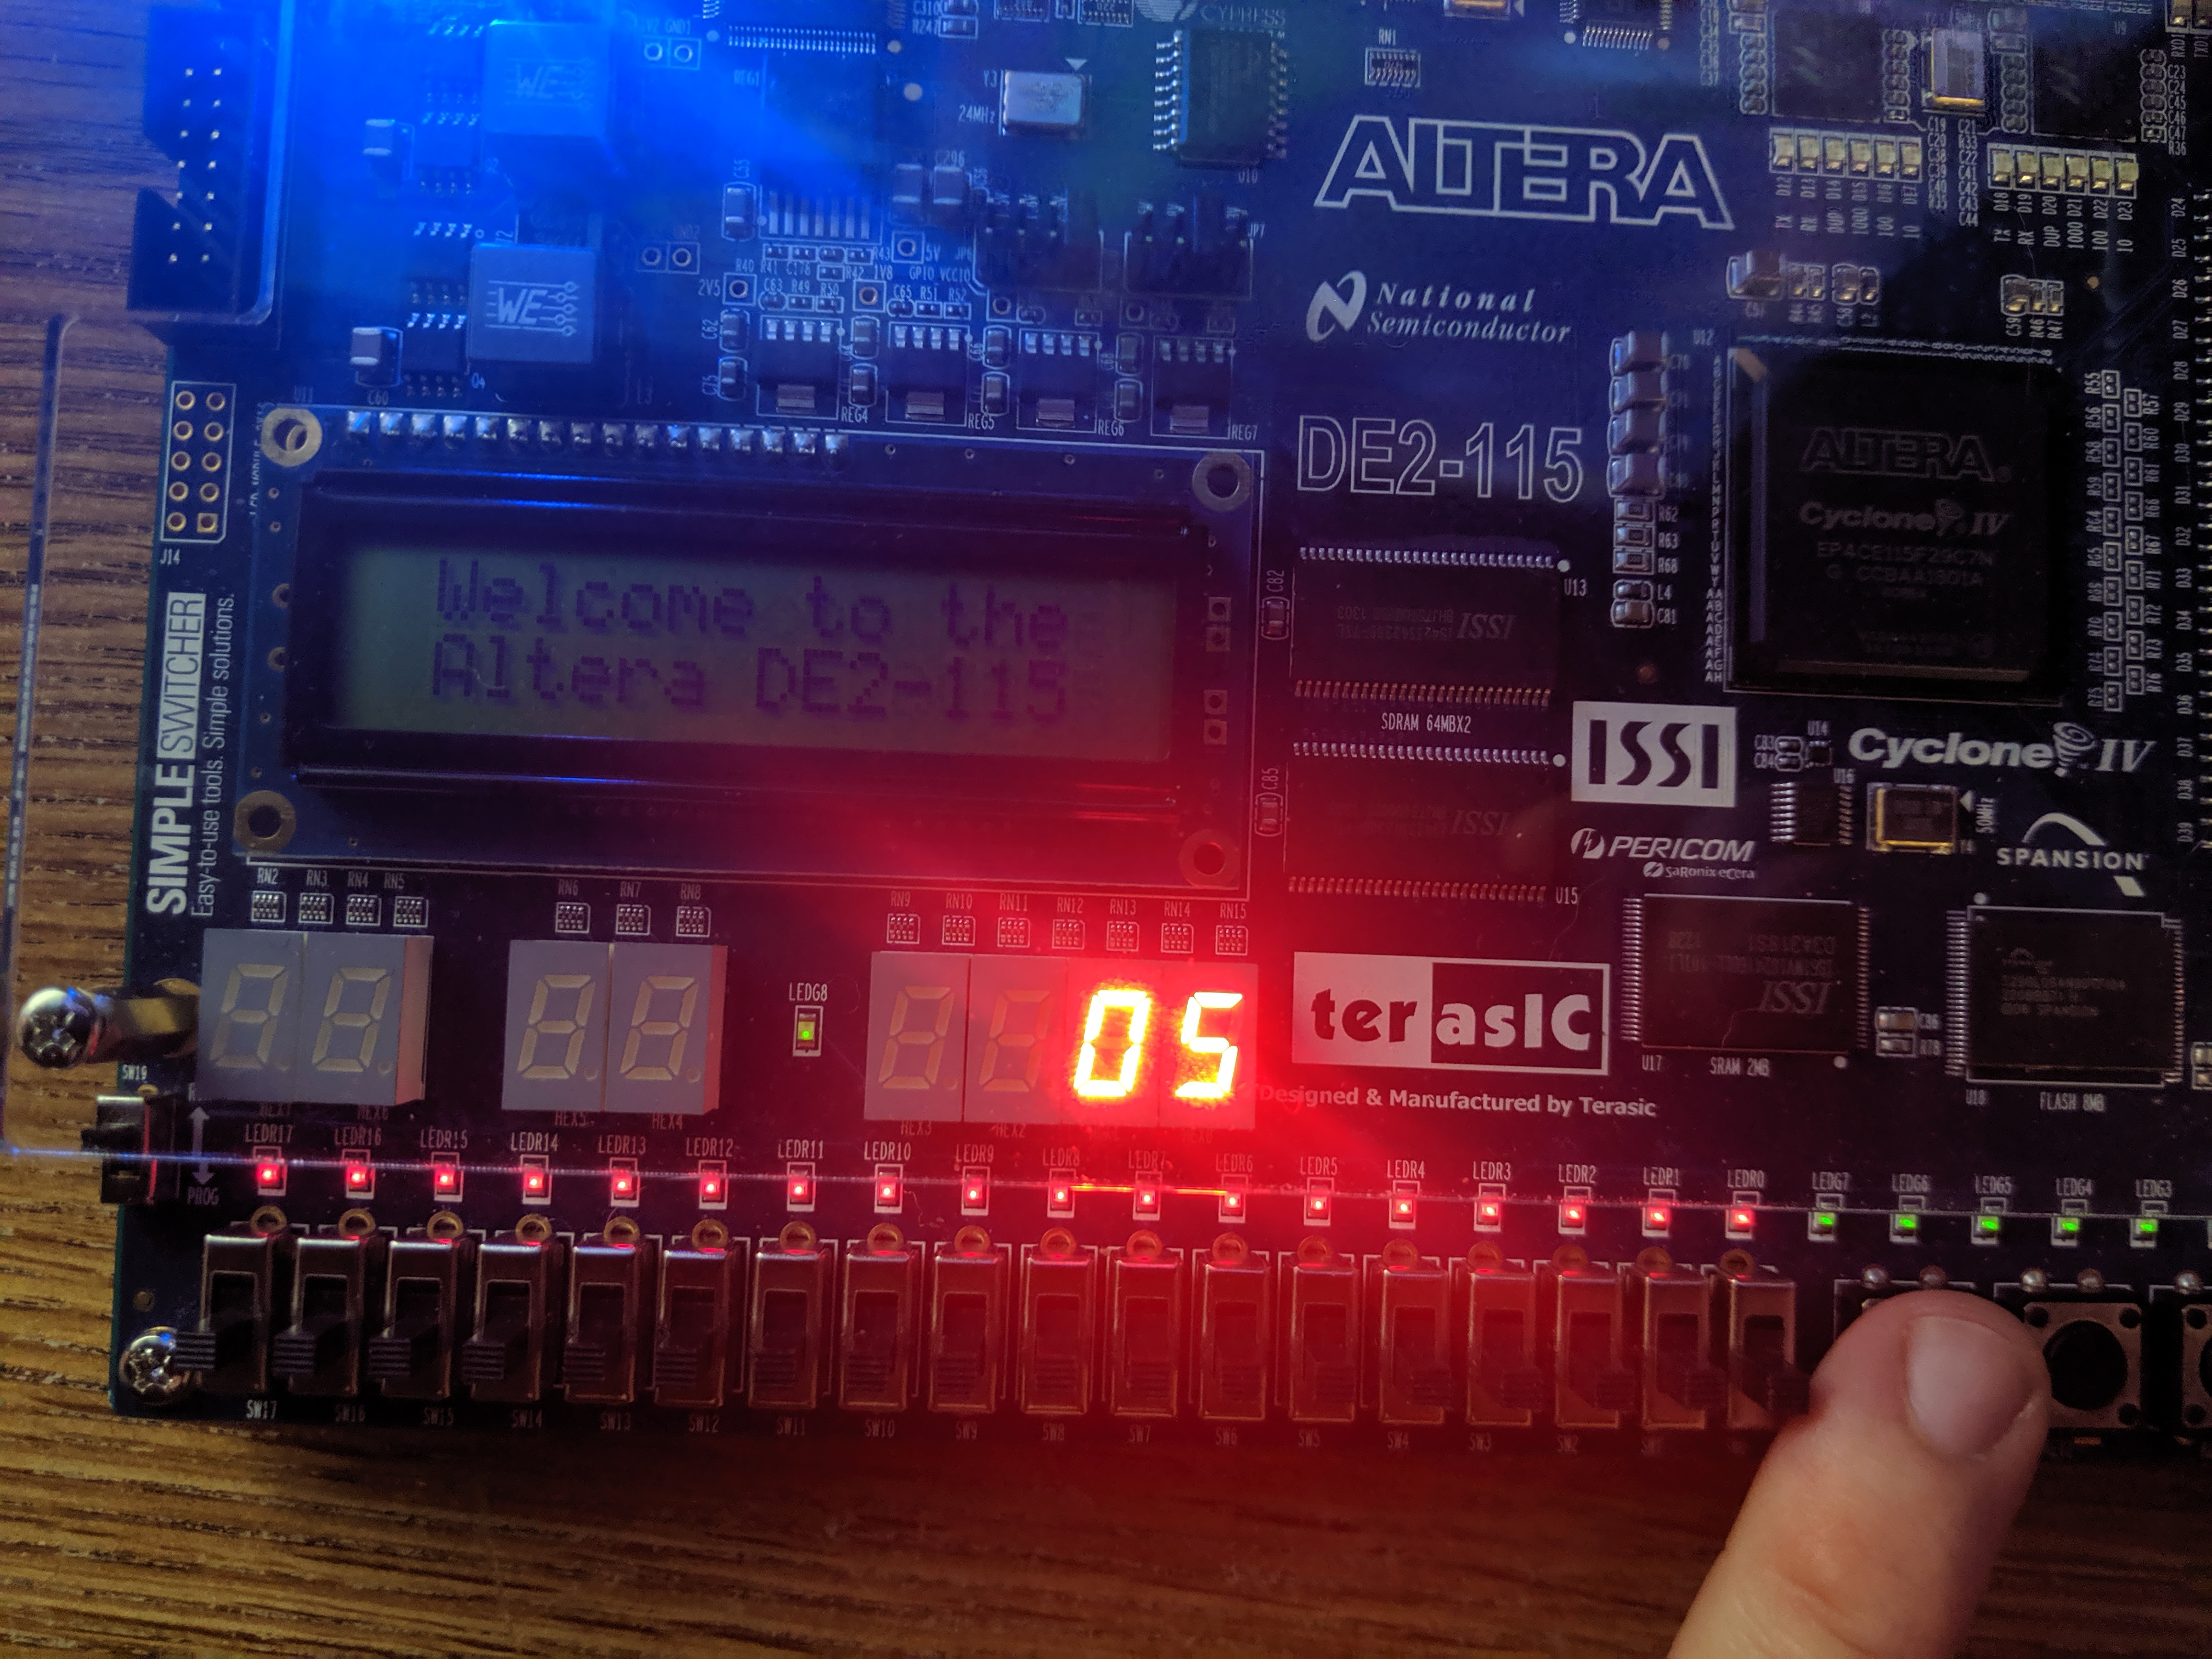
\includegraphics[width=3cm]{Display5.jpg}
				\caption{Display 5}
			\end{subfigure}		
			\begin{subfigure}{3cm}
				\centering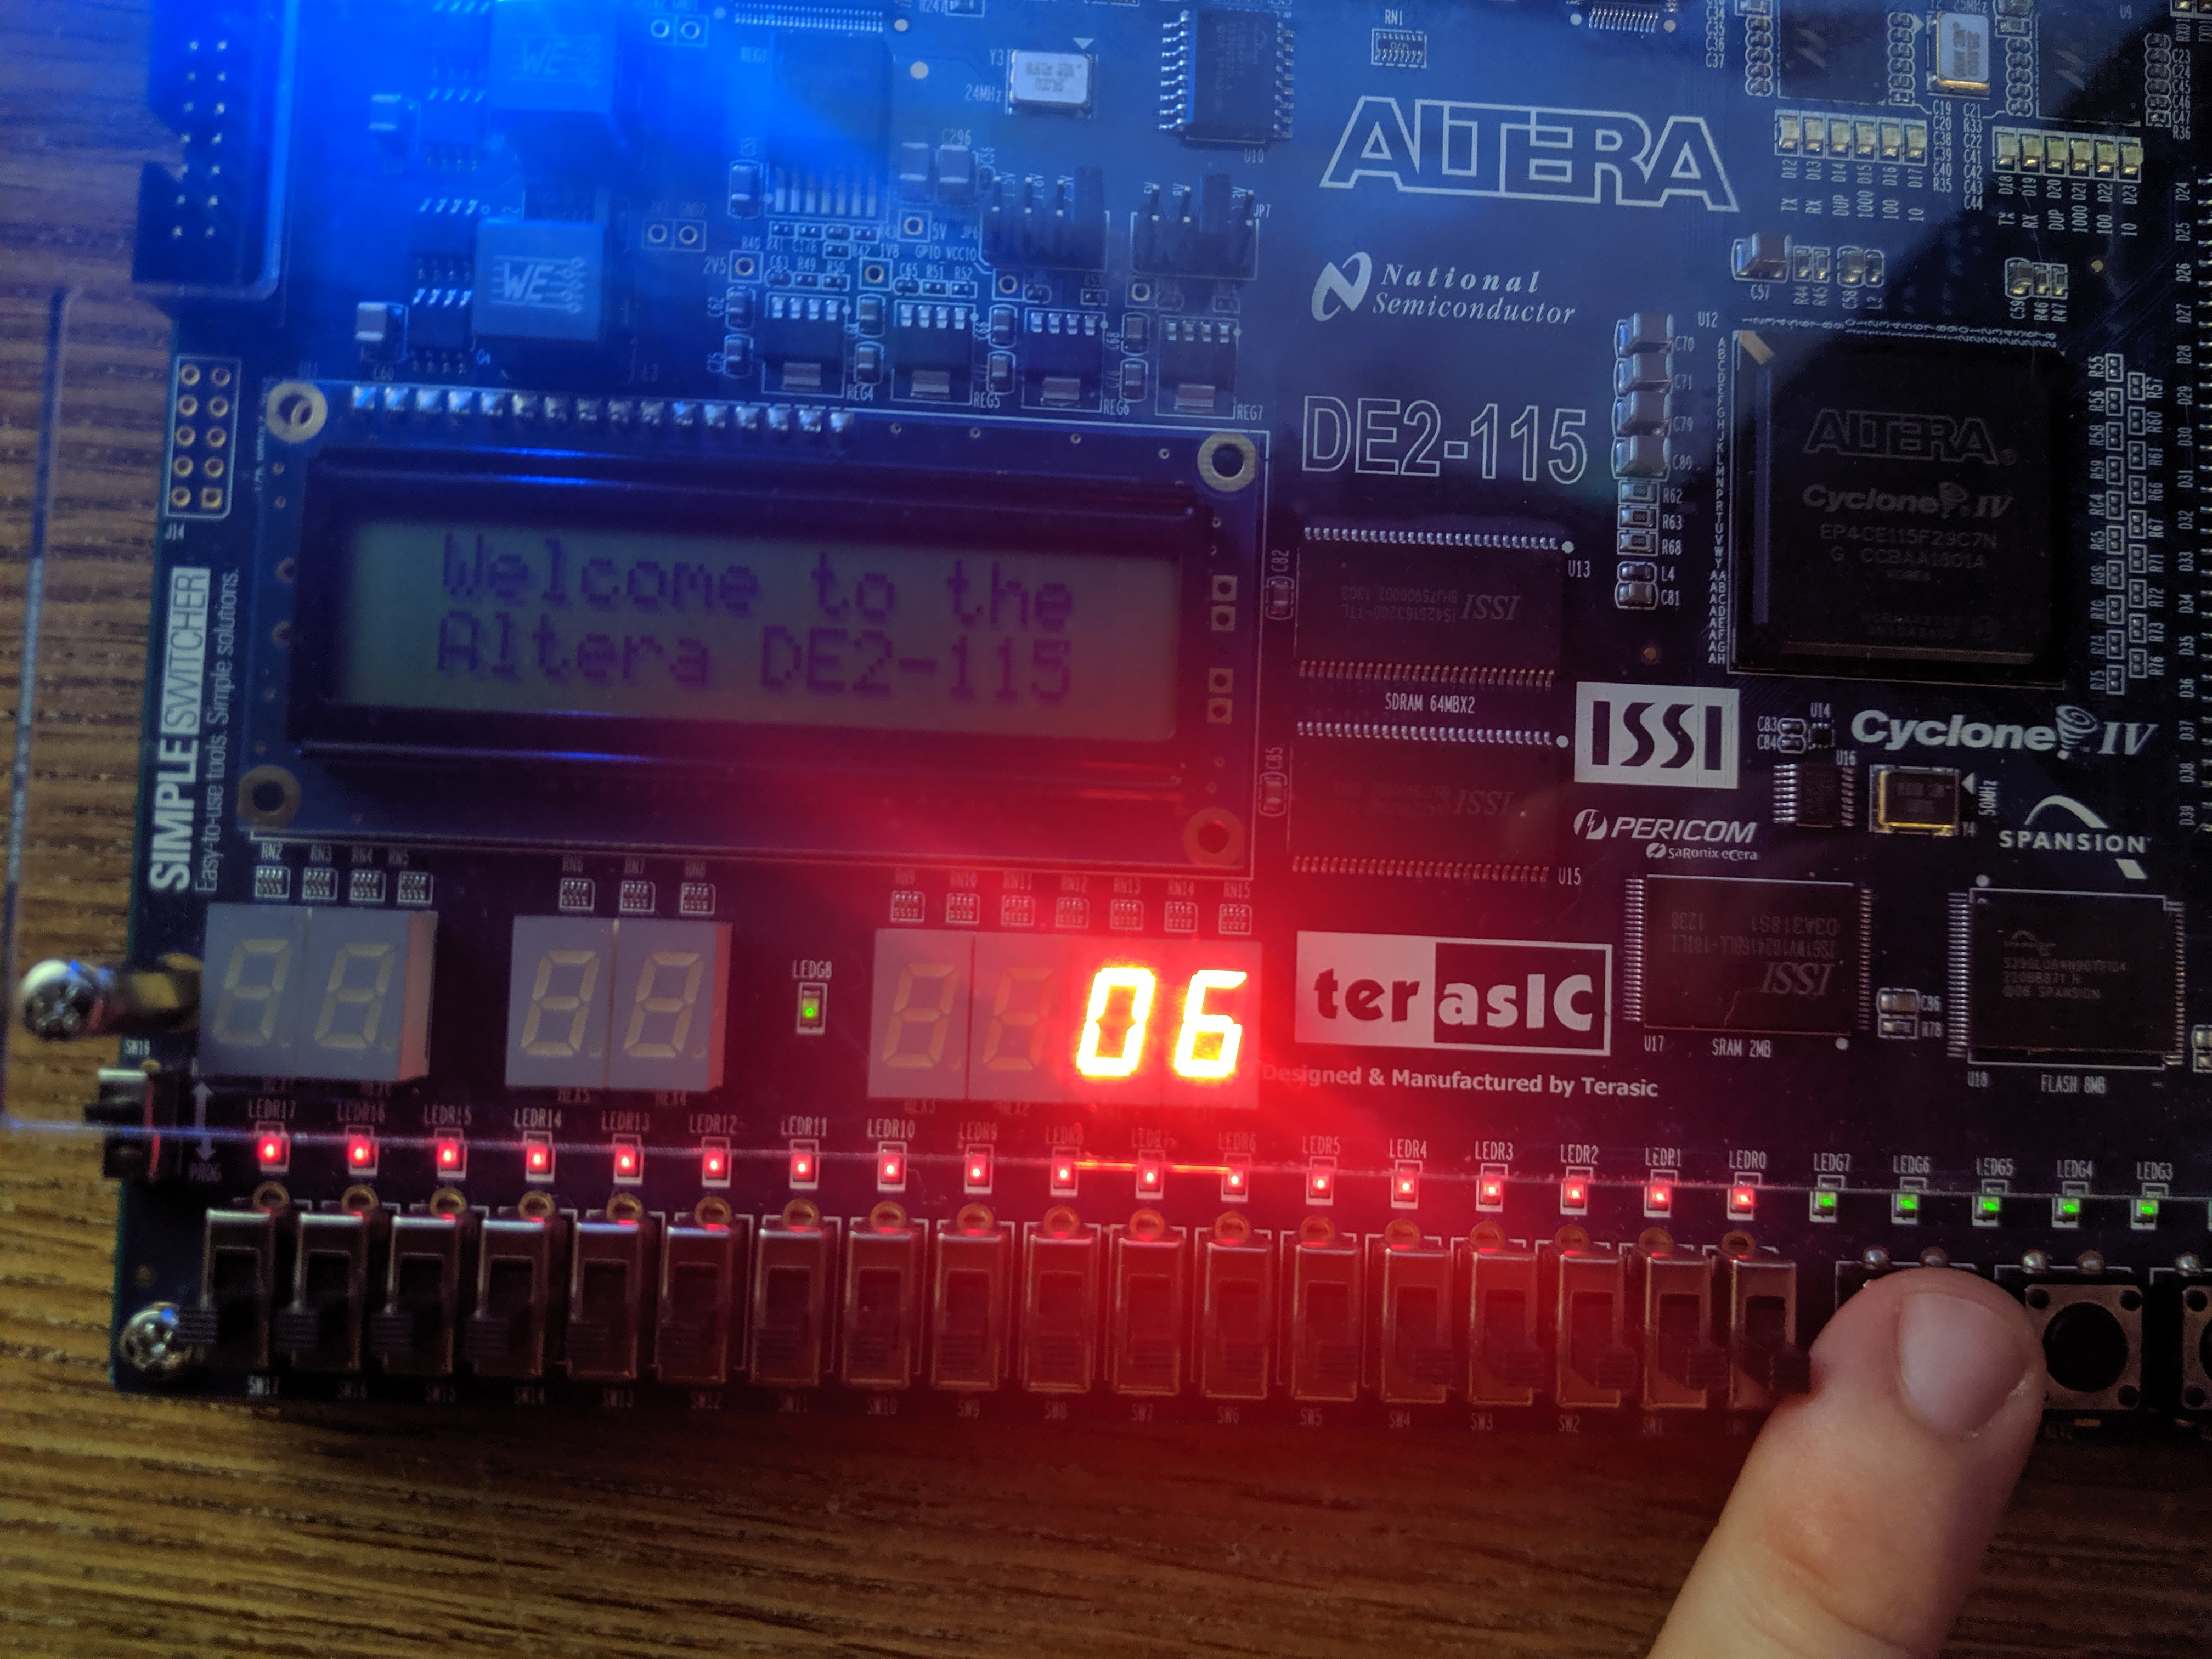
\includegraphics[width=3cm]{Display6.jpg}
				\caption{Display 6}
				
			\end{subfigure}	
			\begin{subfigure}{3cm}
				\centering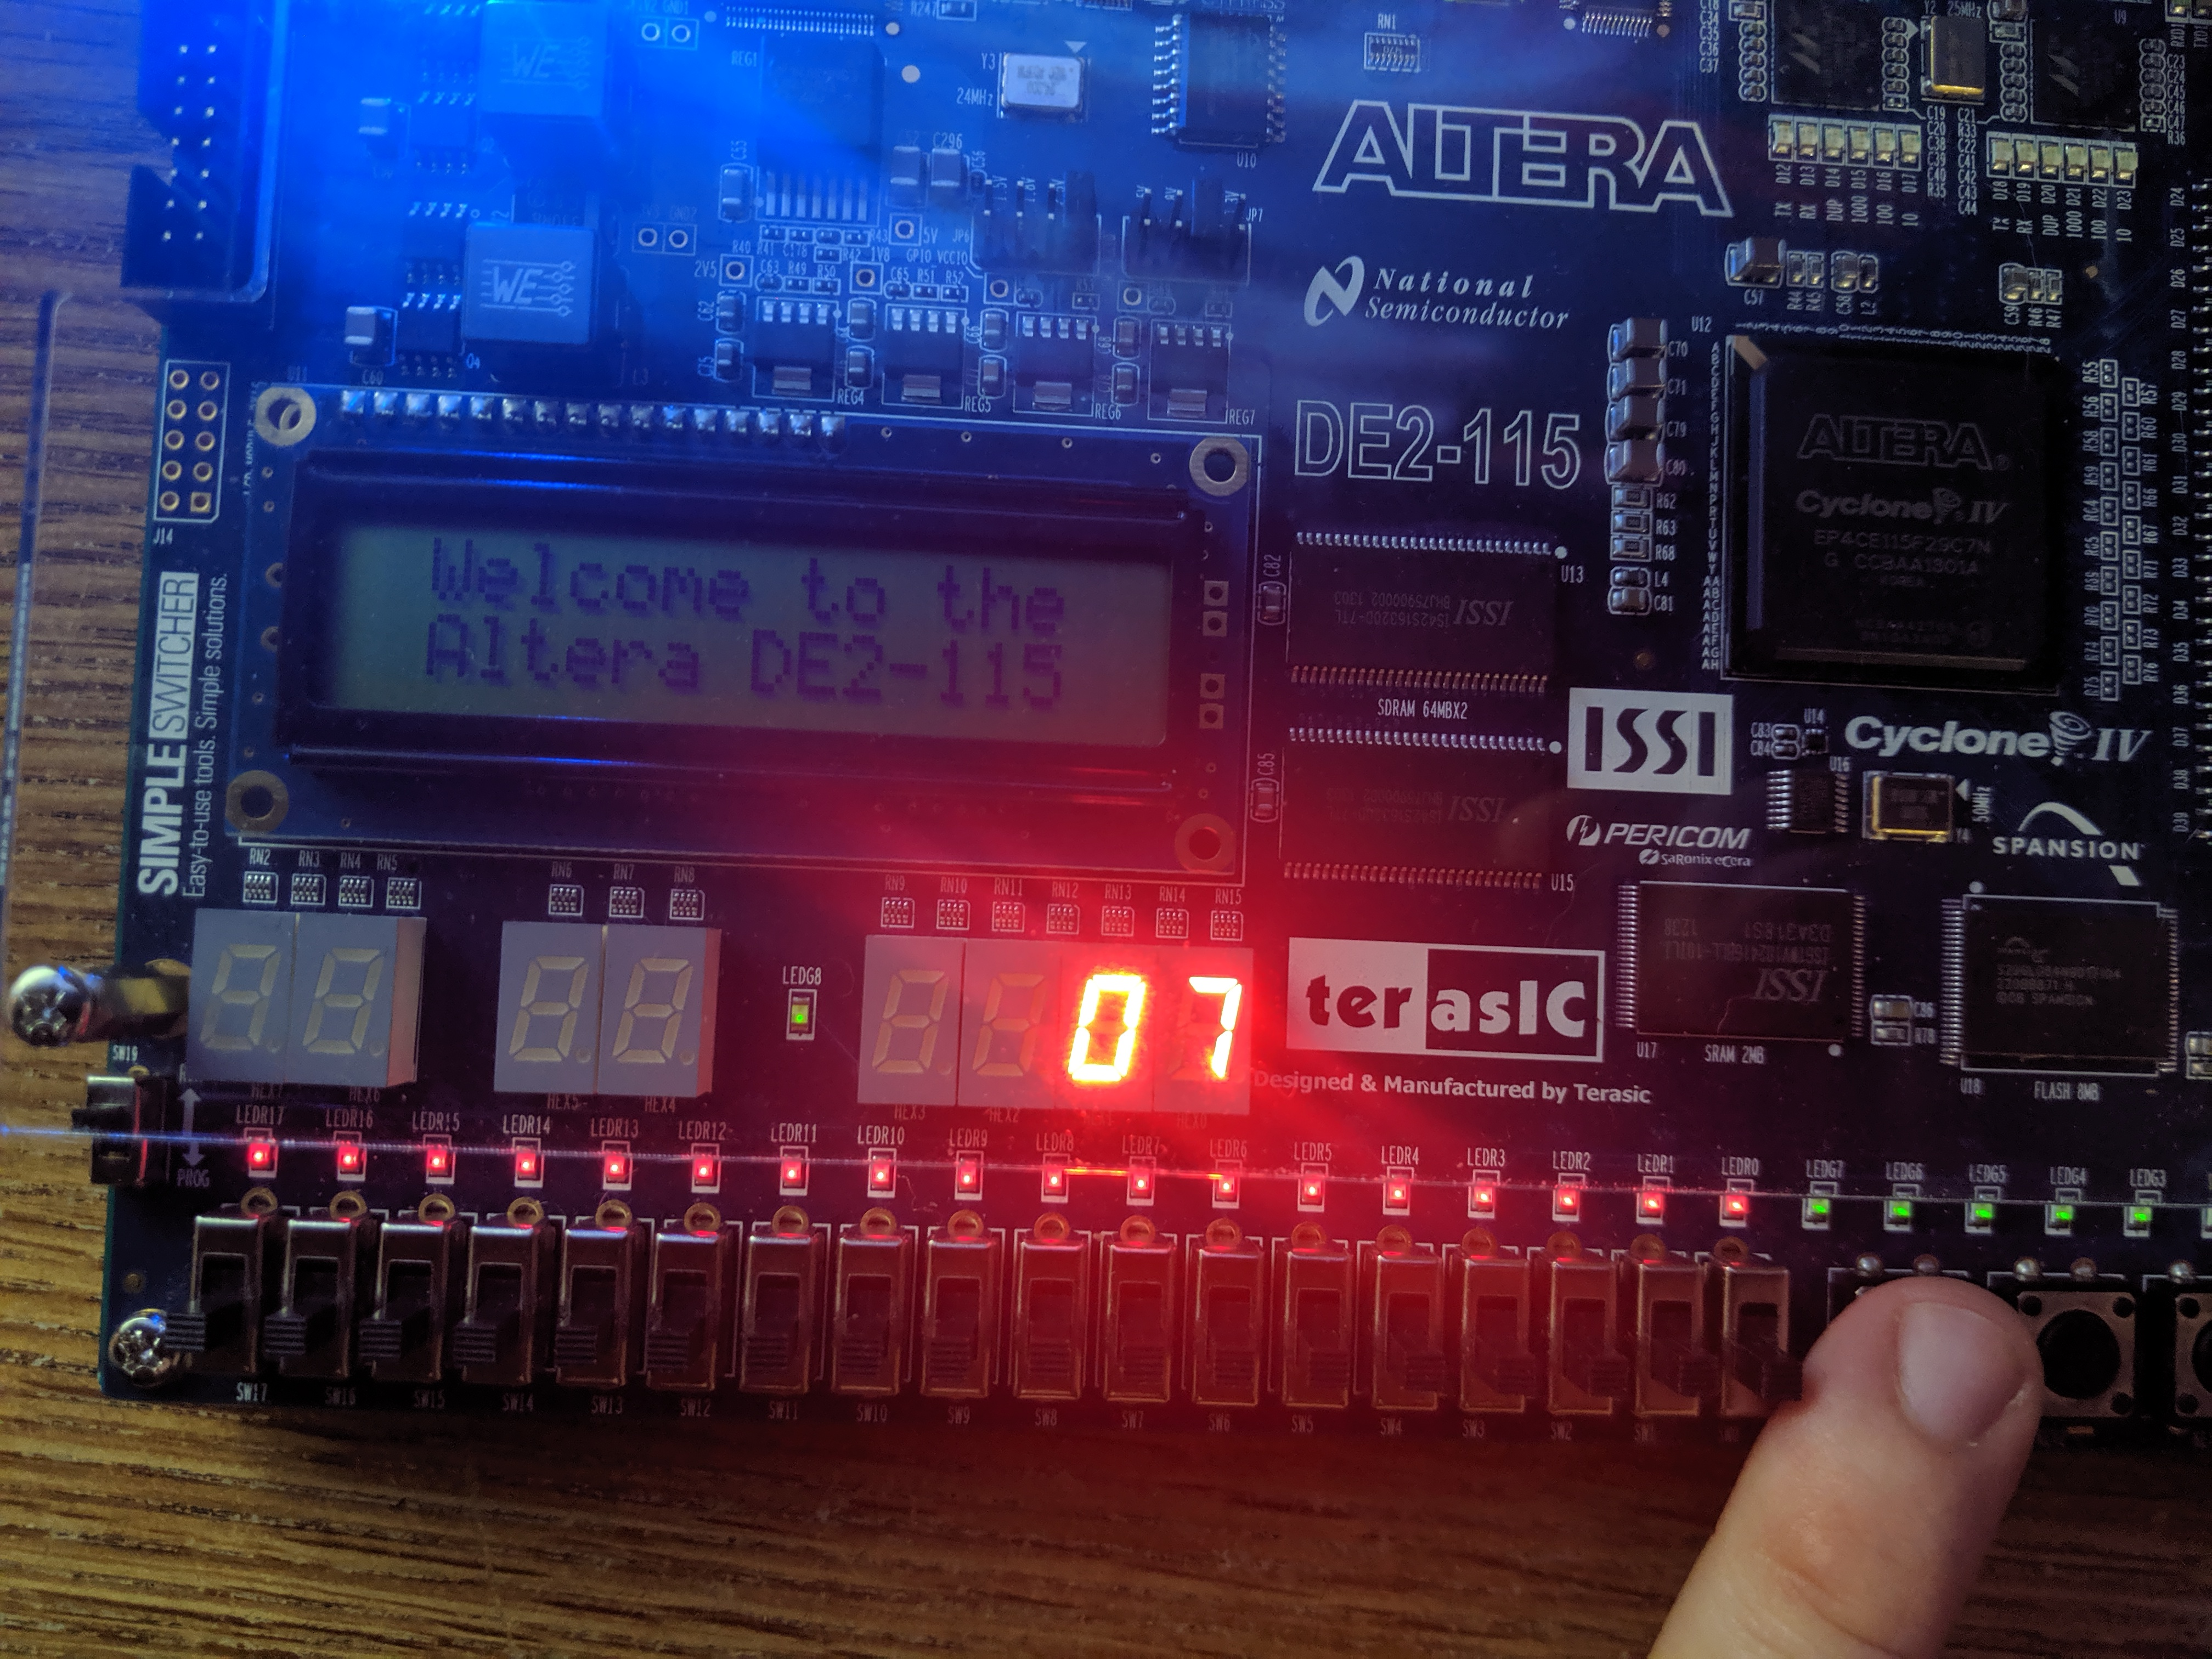
\includegraphics[width=3cm]{Display7.jpg}
				\caption{Display 7}
			\end{subfigure}	
			\begin{subfigure}{3cm}
				\centering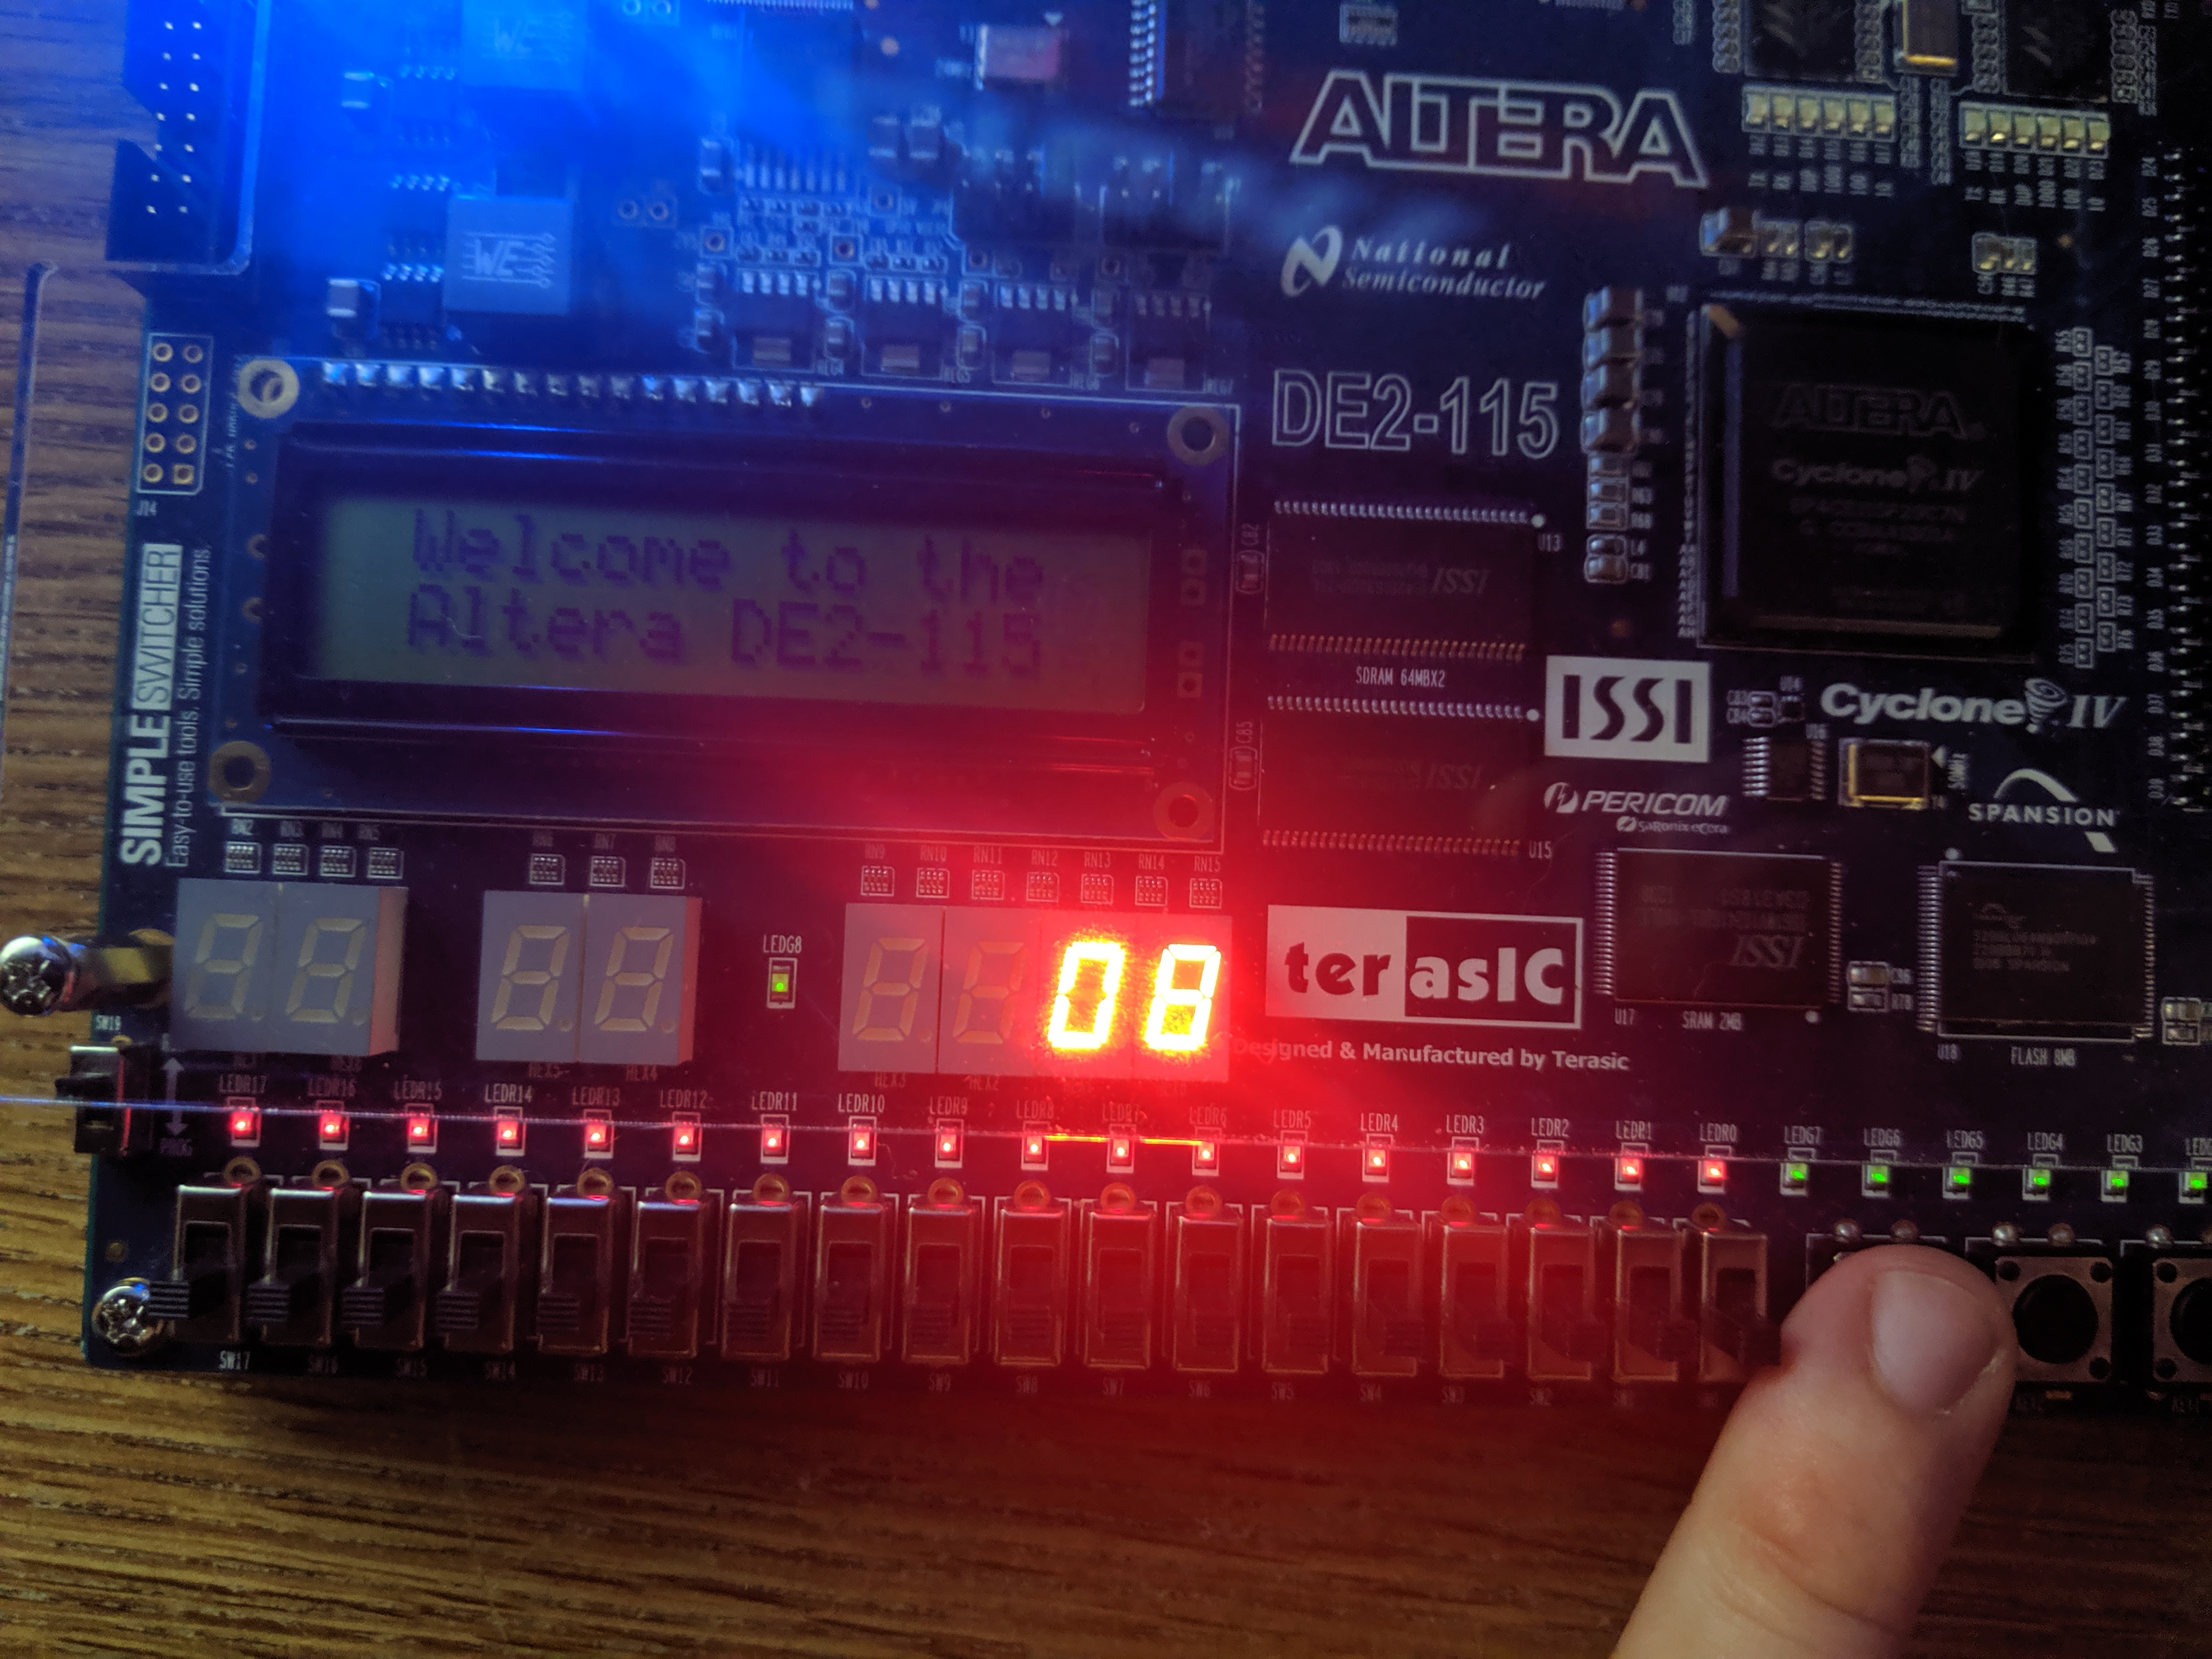
\includegraphics[width=3cm]{Display8.jpg}
				\caption{Display 8}
			\end{subfigure}
			\begin{subfigure}{3cm}
				\centering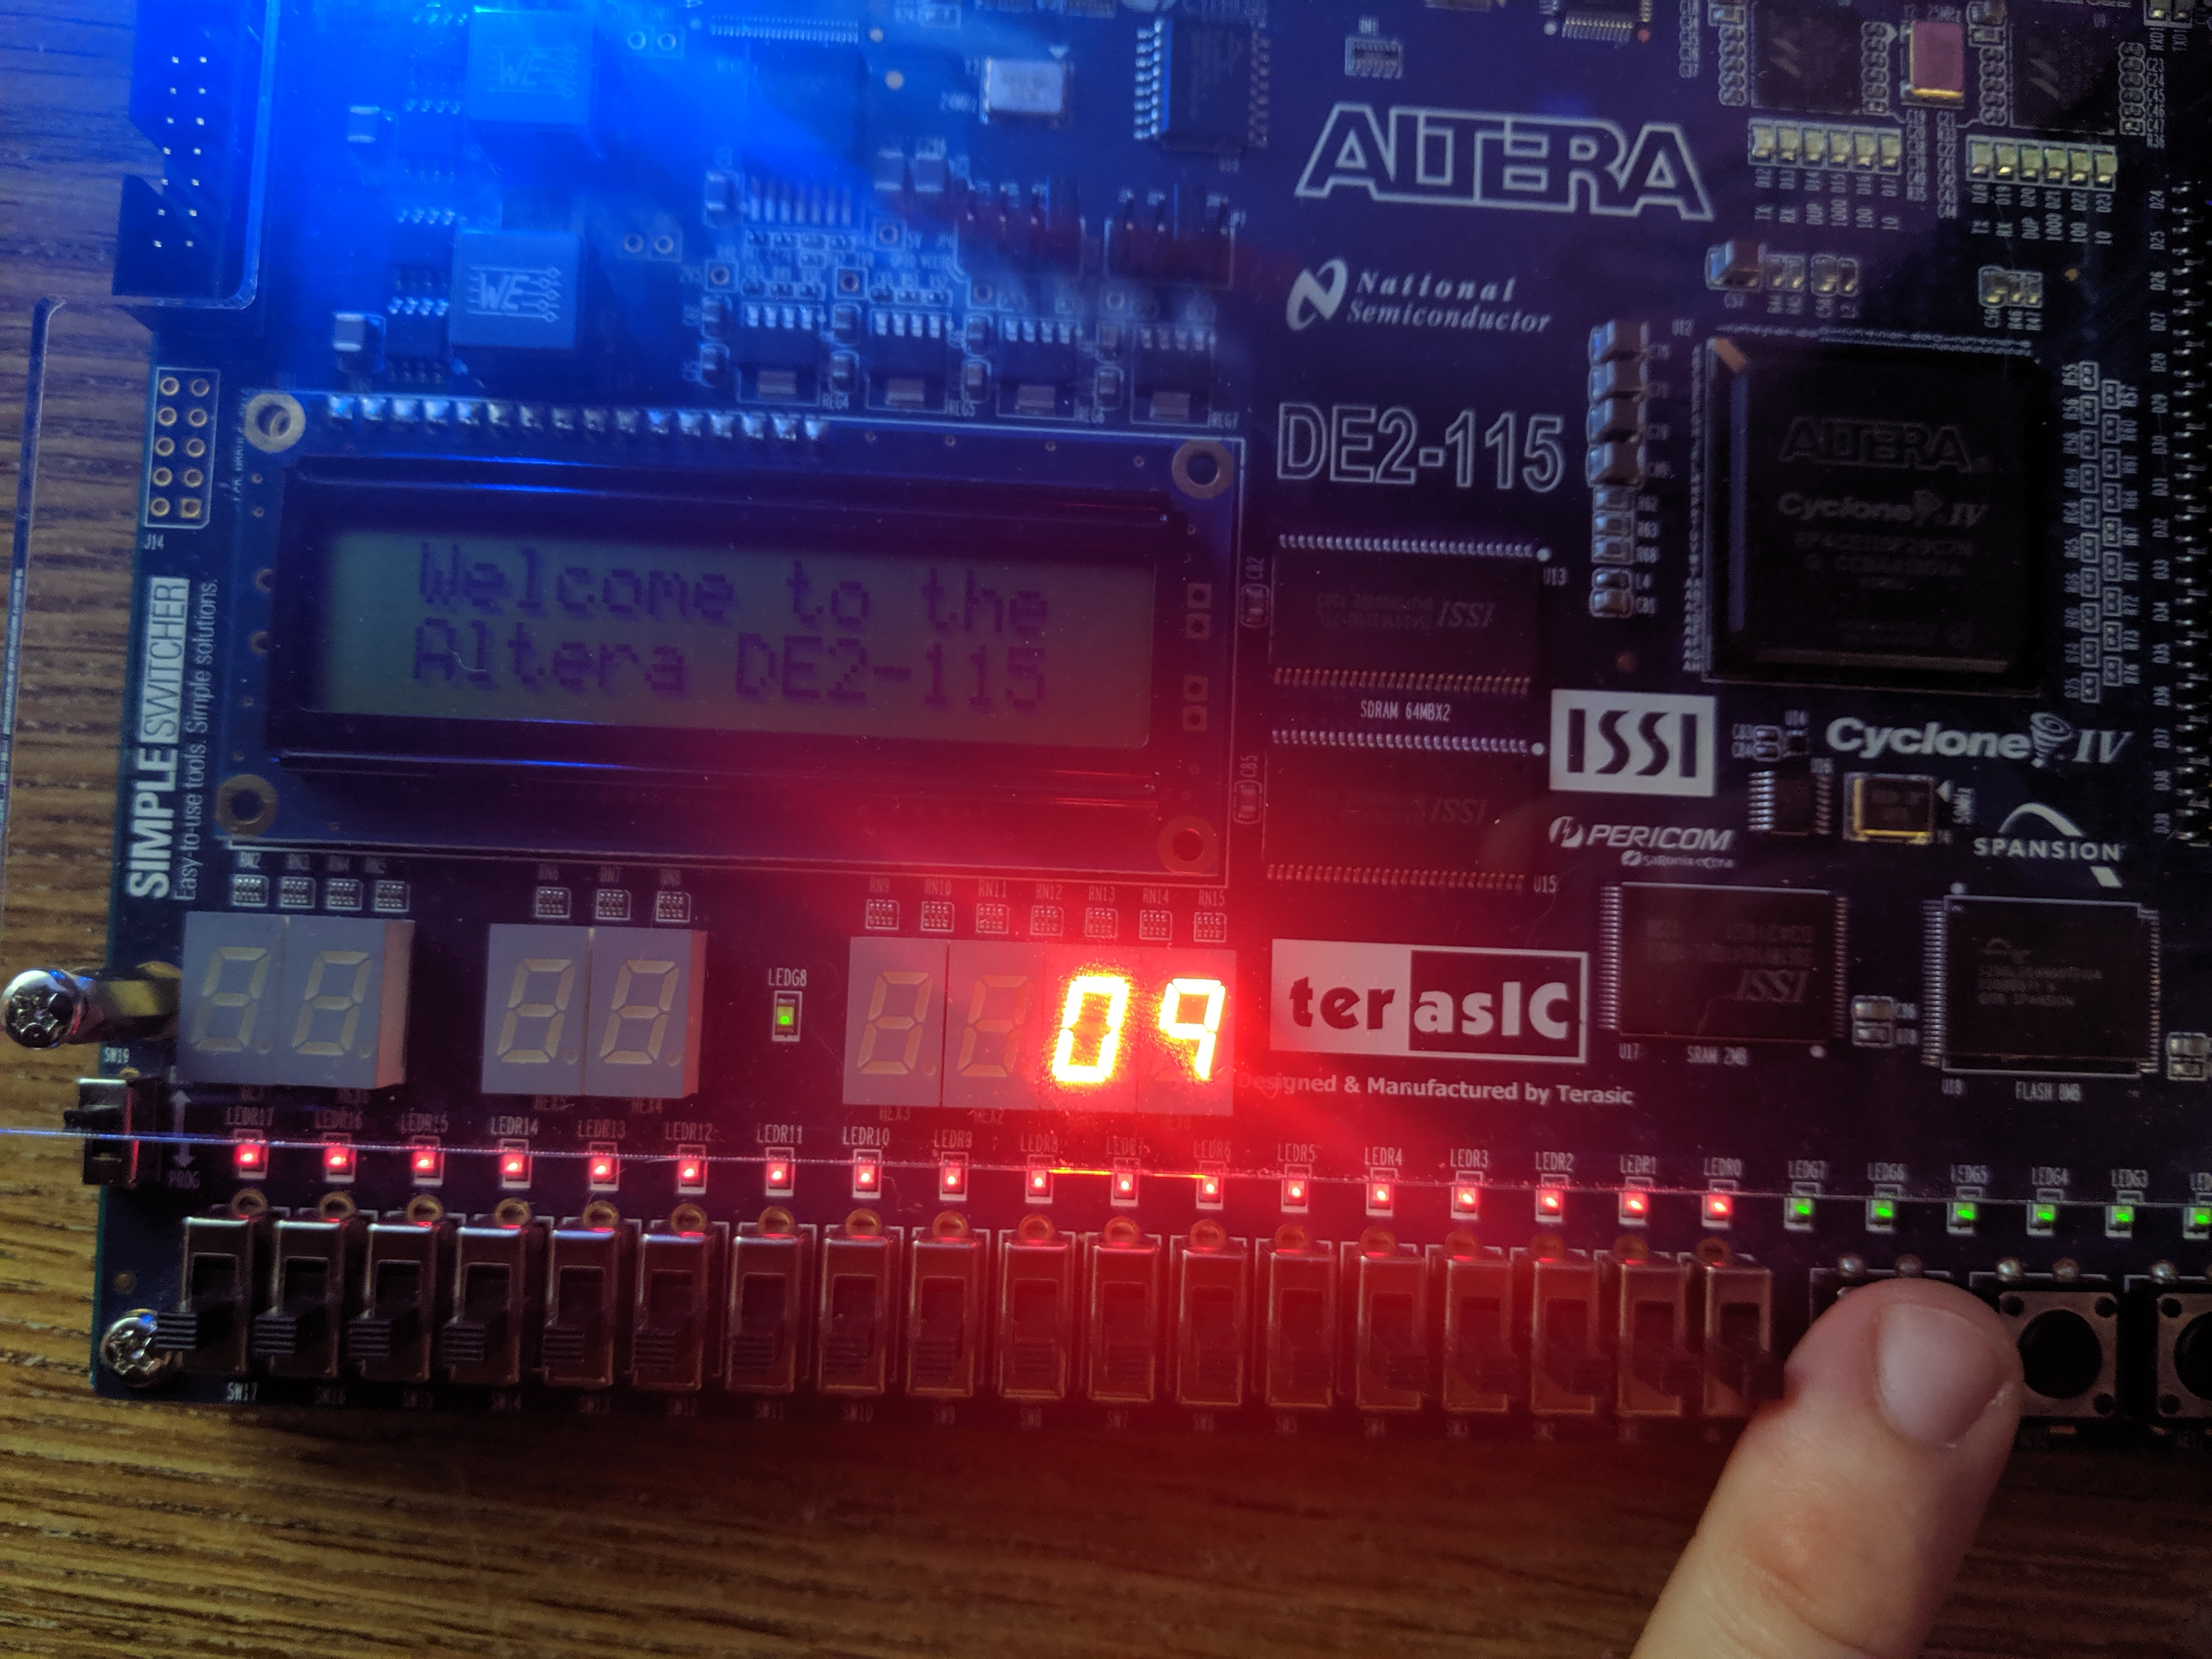
\includegraphics[width=3cm]{Display9.jpg}
				\caption{Display 9}
				
			\end{subfigure}					
			\begin{subfigure}{3cm}
				\centering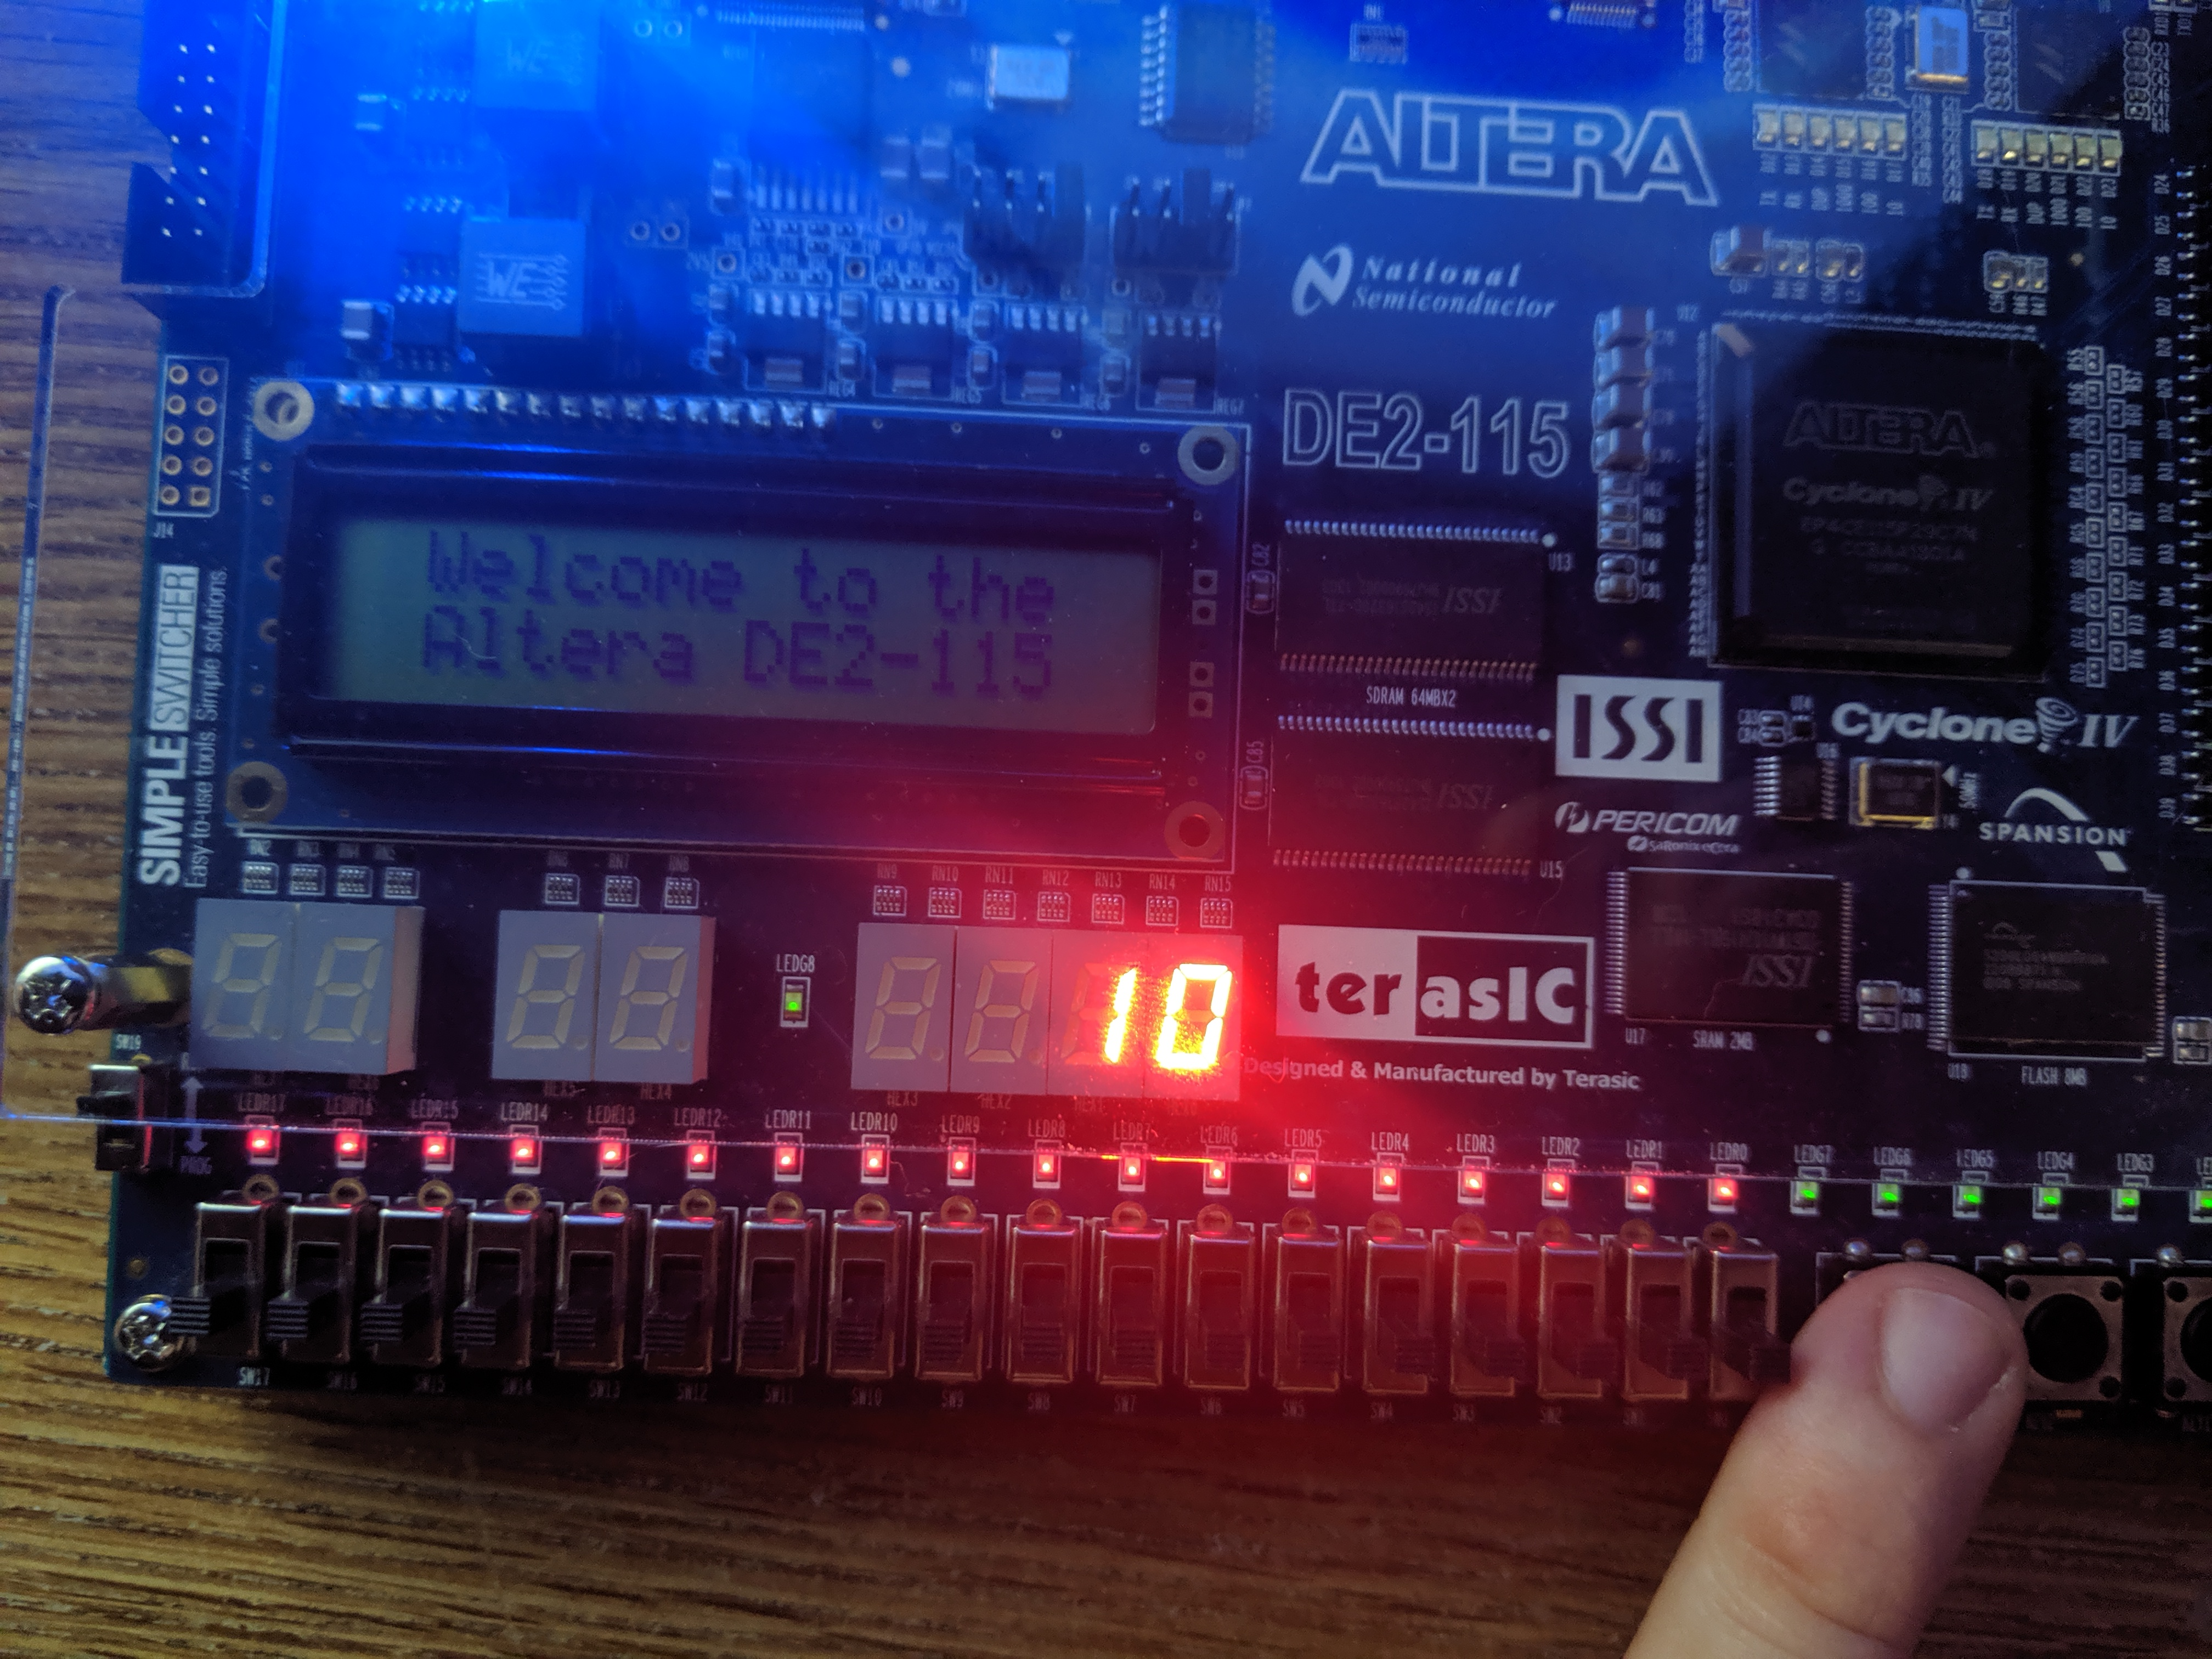
\includegraphics[width=3cm]{Display10.jpg}
				\caption{Display 10}
			\end{subfigure}	
			\begin{subfigure}{3cm}
				\centering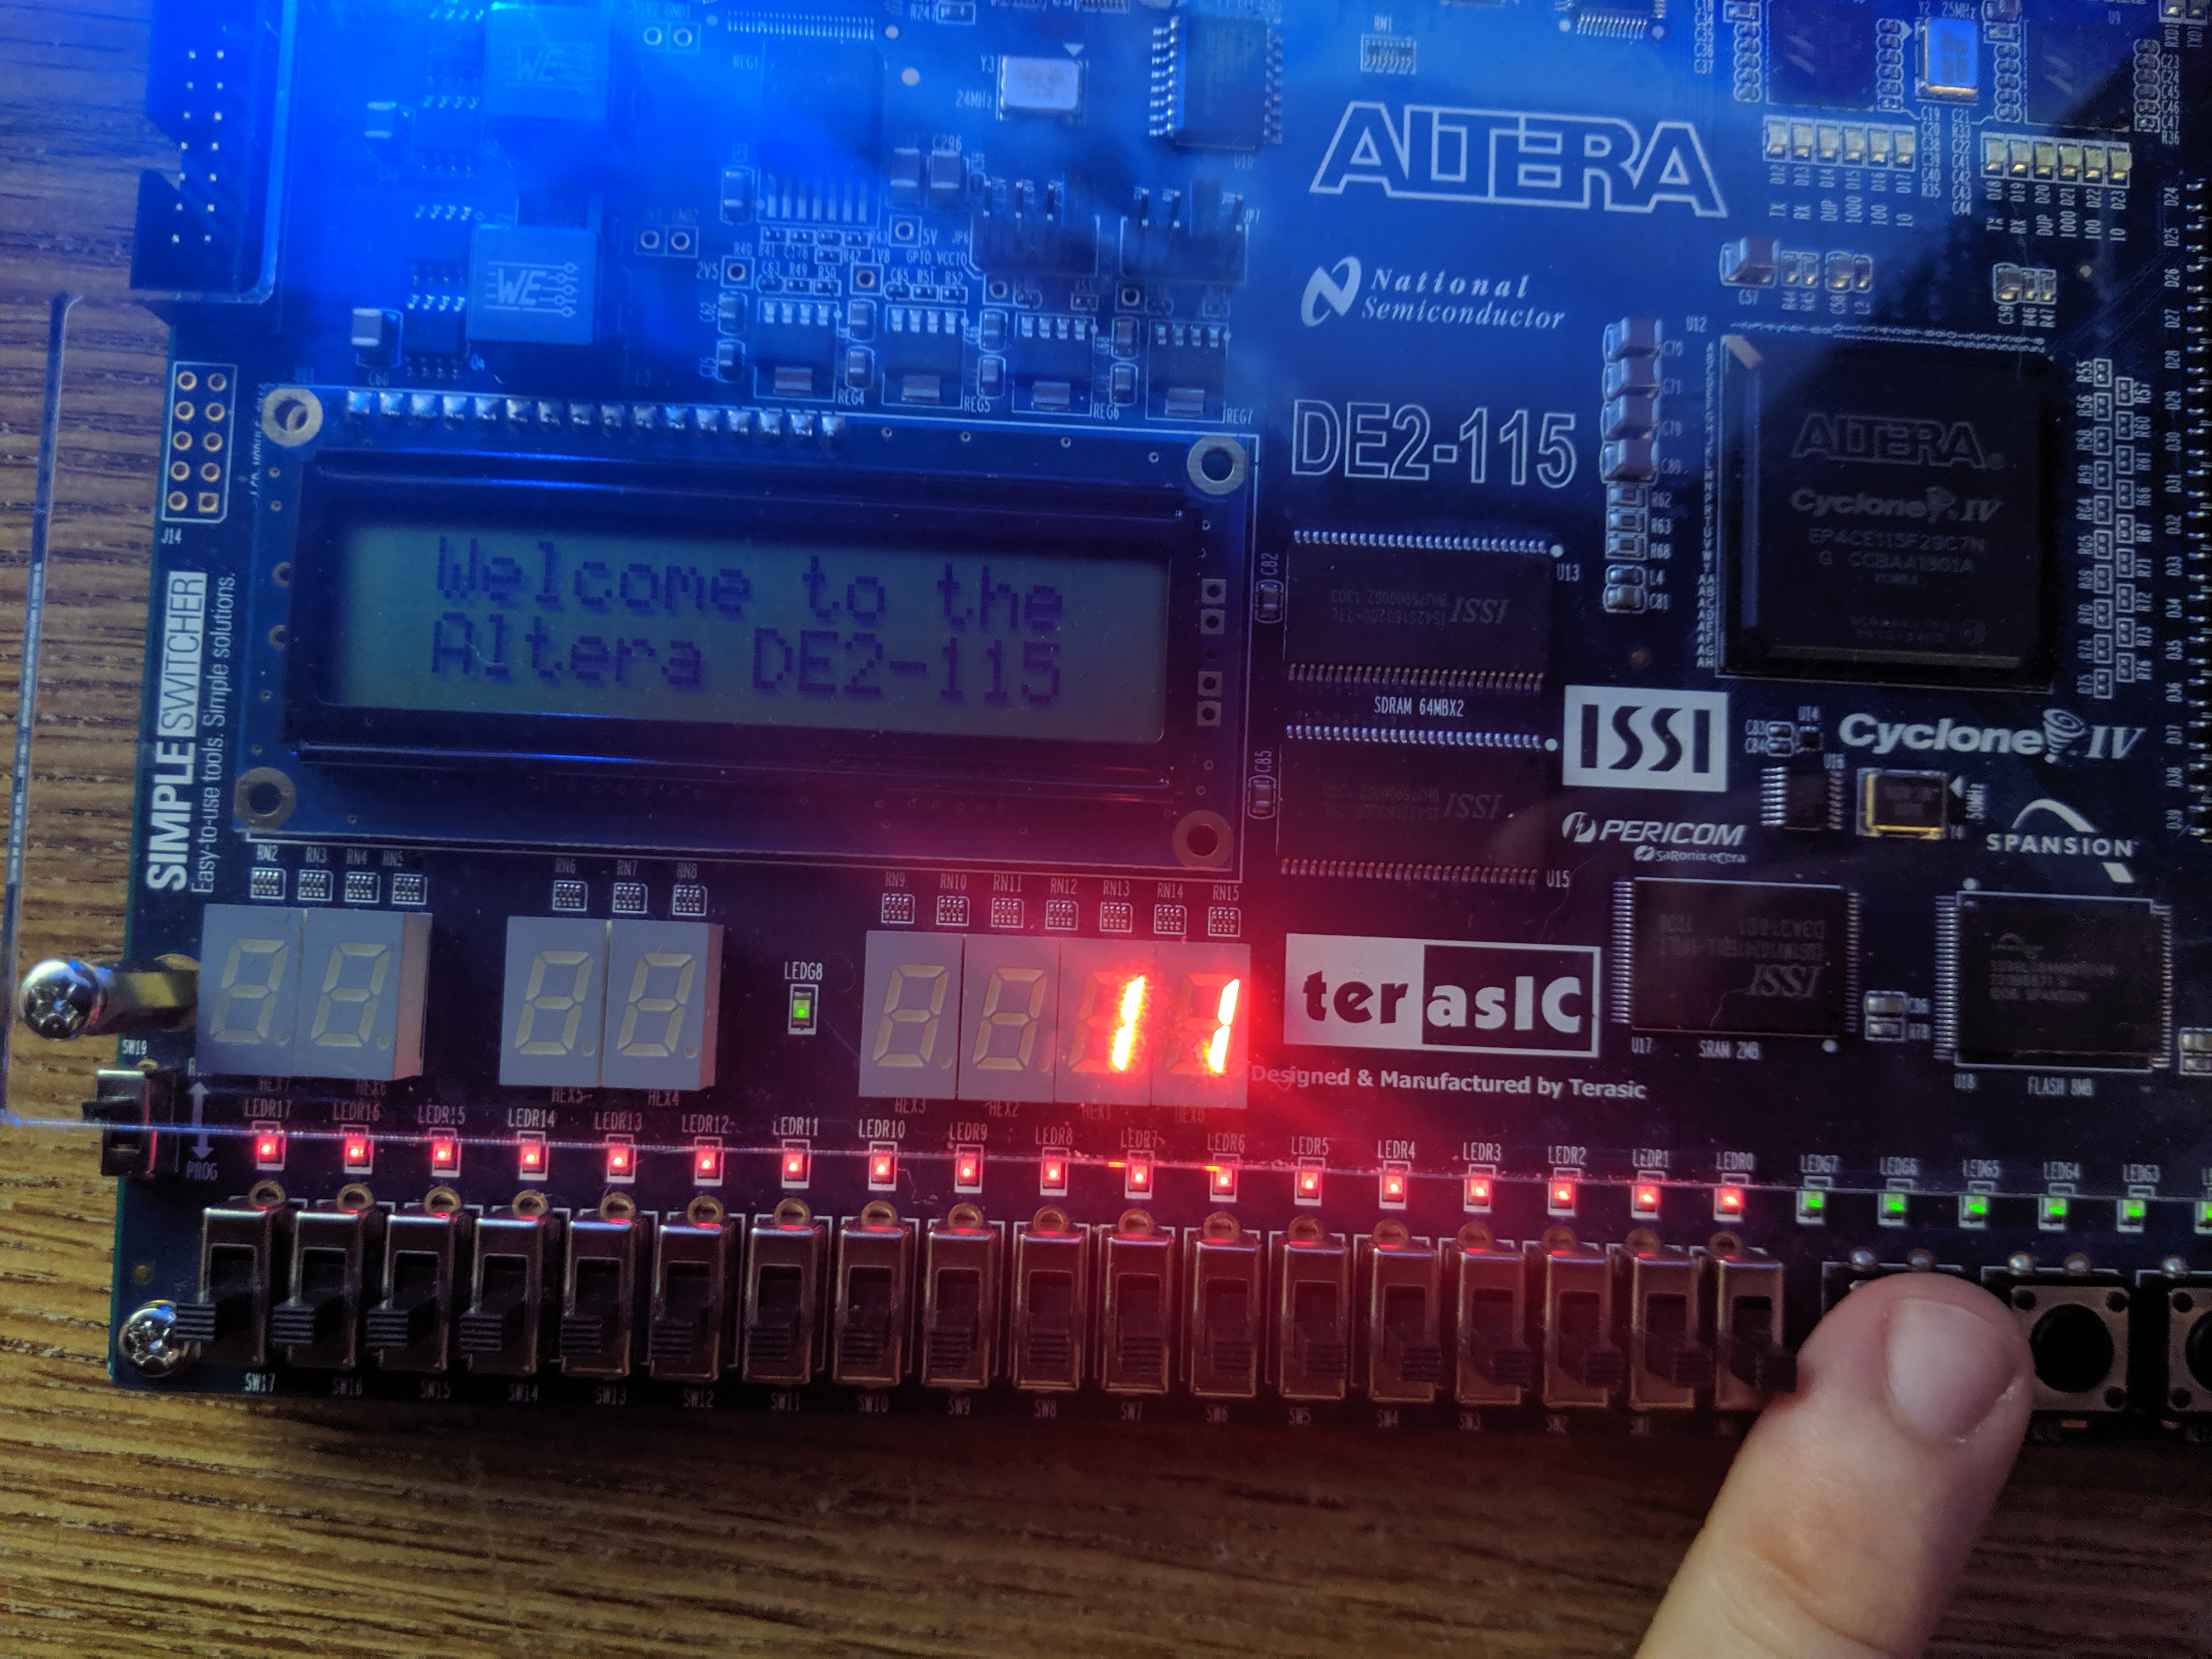
\includegraphics[width=3cm]{Display11.jpg}
				\caption{Display 11}
			\end{subfigure}
			\begin{subfigure}{3cm}
				\centering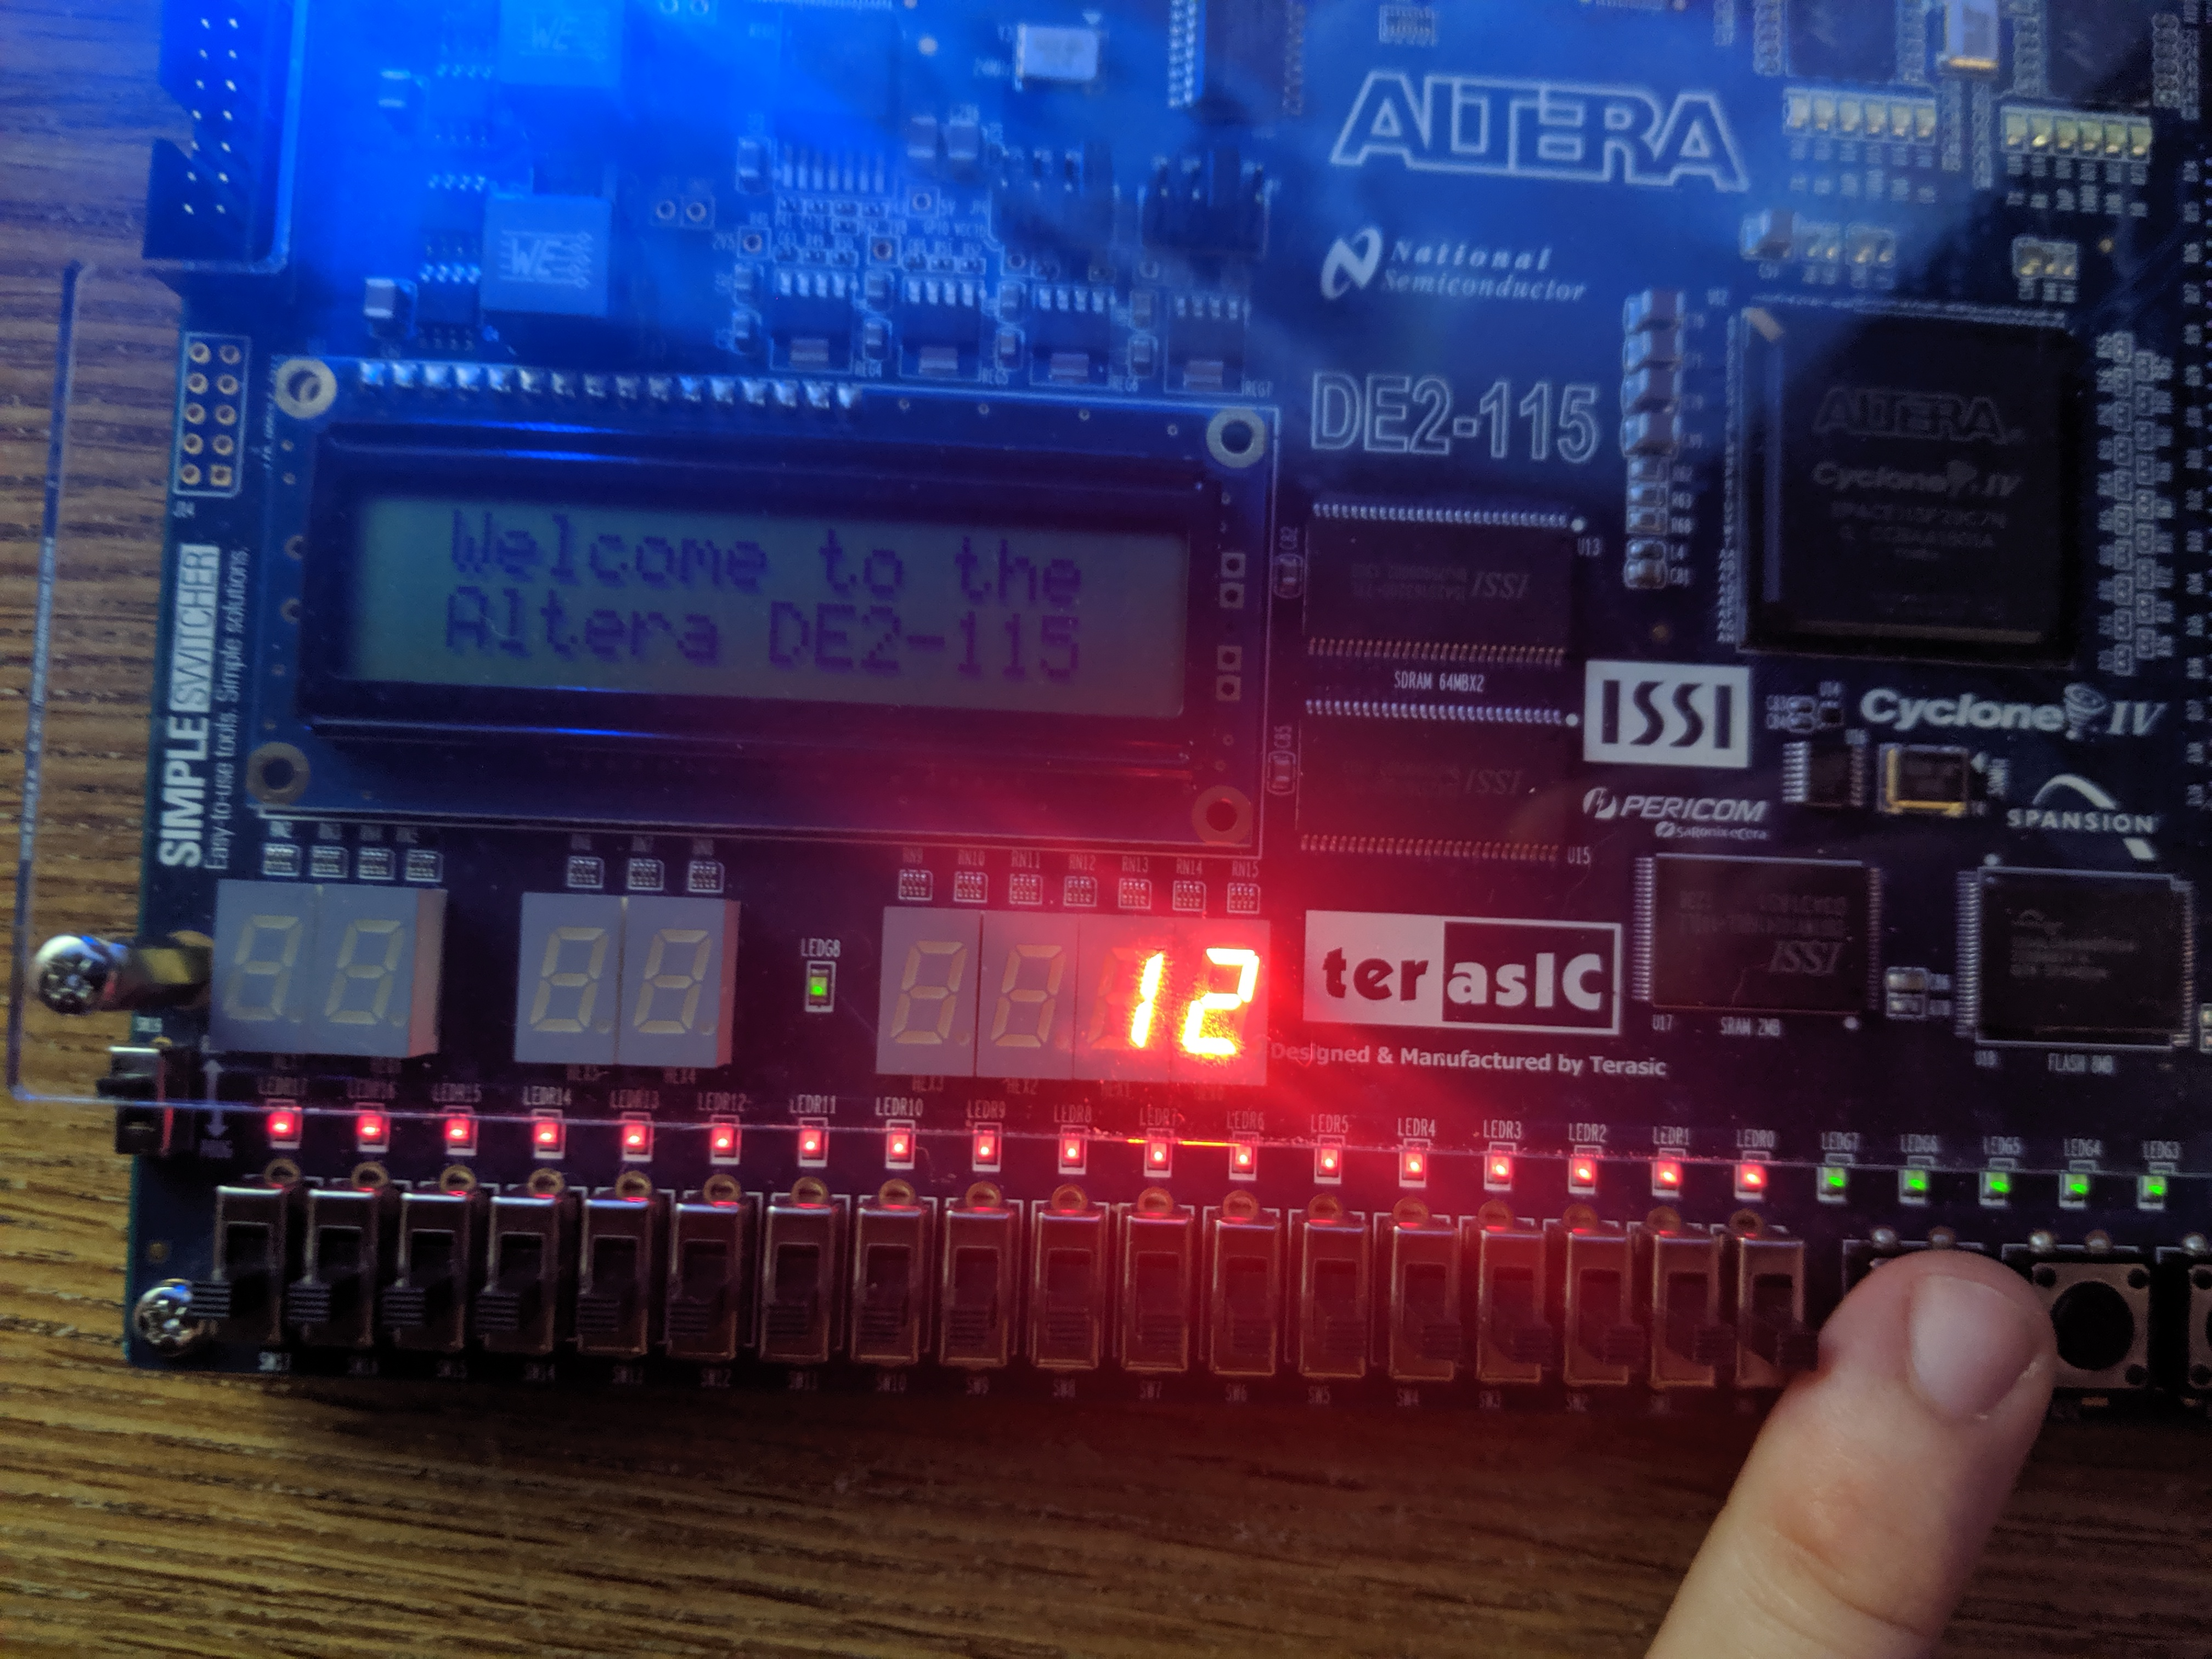
\includegraphics[width=3cm]{Display12.jpg}
				\caption{Display 12}
			\end{subfigure}	
			
			\label{fig:disp}
			\caption{Running 7 Segment Display}
		\end{figure}
		\subsection{Signal Tap Snapshot}
		\begin{figure}[H]
			\centering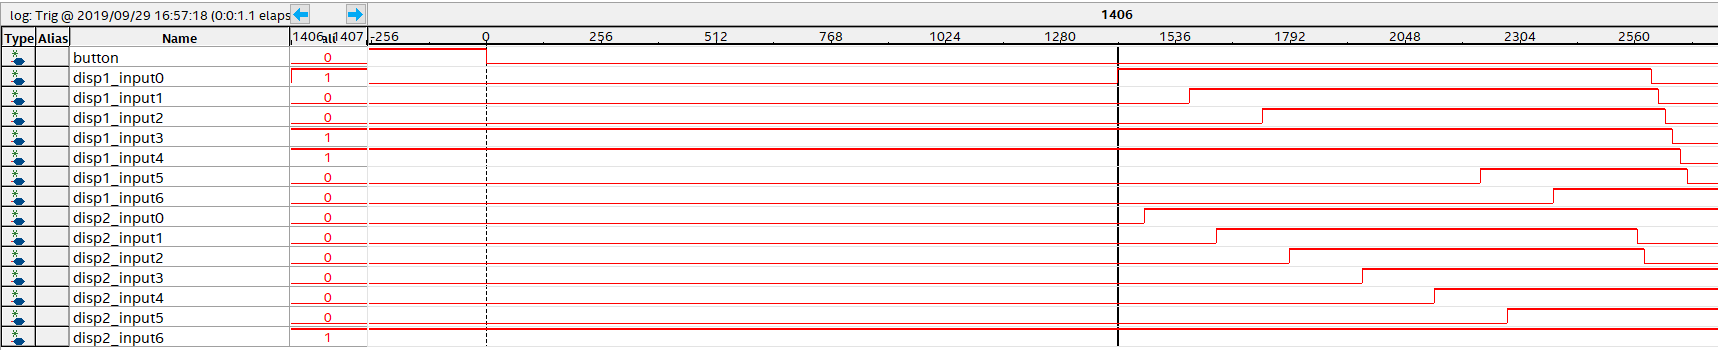
\includegraphics[width=15cm]{Interrupt_Latency.png}
			\caption{Interrupt Latency Measured with Signal Tap}
			\label{la10c}
		\end{figure}
		\subsection{Latency Calculation}
		To calculate the latency based off of Figure \ref{la10c}, we first must calculate the amount of time per cycle using the following equation where $T$ is the time per cycle.
		\begin{equation*}
		f = frequency = 50MHz 
		\end{equation*}
		\begin{align*}
		T = 1/f = 1/50MHz = 0.02\mu s
		\end{align*}
		Once we have the time per cycle we then use that value to calculate the total latency using the number of cycles between the button press and the change in the state of the 7-segment display, which according to the snapshot in Figure \ref{la10c} is approximately 1406 cycles. This calculation is done in the following equation where $n$ is the number of cycles.
		\begin{equation*}
		Latency = T*n = 1406 cycles * 0.02\mu s = 28.12\mu s
		\end{equation*}
		As you can see from the equation above the latency between the button press and the response from the 7-segment display is approximately $28.12\mu s$.
	\section{Conclusion}
	I received your feedback on Homework 1 a few hours after I had finished this project, and would like to note that I did recieve your feedback about using a 7 bit PIO with a std\_logic\_vector instead of using individual bits for the display and so I was not able to incorporate that into this homework but I plan on doing so in the future. I think that the most useful thing that I got out of this assignment was learning how to use the SinalTap tool, and how the system.h file works and what it is used for.
	\clearpage
	\appendix
	\section{\\VHDL Code}
	\lstinputlisting[language=VHDL]{homework2.vhd}
	
	\section{\\C Code}
	\subsection{Headers}
	\lstinputlisting[language=C]{homework2.h}
	
	\subsection{Source}
	\lstinputlisting[language=C]{main.c}
\end{document}